\documentclass[12pt]{article}
\usepackage[letterpaper, margin=1in]{geometry}
\usepackage{graphicx}
\usepackage{subcaption}
\graphicspath{{./images/}}
\usepackage{hyperref}
\usepackage{parskip}
\usepackage{amsmath}
\usepackage[framed, numbered]{matlab-prettifier}
\lstset{inputpath=../}
\usepackage{titlesec}

\titleformat*{\section}{\large\bfseries}
%\allowdisplaybreaks

%
\makeatletter
\setlength{\@fptop}{0pt}
\makeatother
%

\title{ELECENG 3CL4 Lab 3 Report}
\author{
    Aaron Pinto \\
    pintoa9 \\
    L02
    \and
    Raeed Hassan \\
    hassam41 \\
    L02
}

\begin{document}

\maketitle
\clearpage

\section*{Member Contributions} % copied from lab doc
Both group members contributed an even amount to both the exercises and the report. Both members went through the exercises together and contributed to all sections of the report.

\section*{Objective}
To design a proportional controller and a proportional controller with velocity feedback for the DC motor servomechanism, and explore trade-offs involved in the selection of the controller parameters and their impact on transient and steady-state responses of the control system.

\setcounter{section}{2}
\section{Experiment: Qualitative Trade-offs in Rise-time, Steady-State Error, Overshoot, and Settling Time for a Proportional Controller}
% talk about measurement procedure
In order to measure the peak overshoot (with respect to the final value) and steady state error, we measured the delta between the first peak and the steady state value using the peak finder tool for the peak and a cursor for the steady state value. The settling time measurement was performed by moving a cursor to the point at which the last oscillation was ending and the plot showed a straight line after. The time value shown on the cursor table was then taken as the settling time. The rise time was measured using a cursor as the time from 0 to the first instance of when the output reached the steady state value. We tried the "Bilevel Measurements" tool, but we found it to be inaccurate, though it did give us an approximation of where our values should be.

\begin{table}[h!]
\centering
\begin{tabular}{|c|c|c|c|c|c|c|} \hline
    $k_p$ & 0.5 & 1 & 2 & 3 & 4 & 5 \\ \hline
    peak overshoot (\%) & 0.7 & 38.4 & 54.7 & 65.7 & 75.3 & 82.4 \\ \hline
    steady-state error (deg) & 26.89 & 8.09 & 5.10 & 3.69 & 2.64 & 1.93 \\ \hline
    settling time (sec) & 0.336 & 0.469 & 0.618 & 0.771 & 0.881 & 1.067 \\ \hline
    rise time (sec) & 0.336 & 0.125 & 0.100 & 0.076 & 0.064 & 0.058 \\ \hline
\end{tabular}
\caption{\label{table:exp1_measurements}Measurements for Experiment 1}
\end{table}

% observations or something here
We measured values for the peak overshoot, steady-state error, settling time, and rise time at $k_p$ values of 0.5, 1, 2, 3, 4, and 5. The measurements are presented in Table \ref{table:exp1_measurements}. The figures for the step response plots are shown in Appendix \ref{appendix:exp1fig}. As we increased the proportional gain, we observed that the peak overshoot percentage increased, the steady state error decreased the settling time increased, and the rise time decreased. This matches our expectations from the theoretical calculations and investigations in the pre-lab and the behaviour that we have observed in previous labs. % The settling time increases because the system is underdamped and as we increase $k_p$ the real part of the poles decrease (the poles approach the $j\omega$-axis), and the the constant $\tau_m$ is defined as $\frac{1}{Re(pole)}$ and for a moderately underdamped system, $T_s$ is $\approx 8\tau_m$.

% You should  plot the positions of the poles of the closed-loop transfer function from R(s) to Θ(s), for each of the chosen values of kp, and you should comment on how the transient  performance of the system can be predicted from these closed-loop pole positions. To assist you in plotting the closed-loop pole positions, observe that we can plot an x at the point a+jb in the s-plane using the Matlab command plot(a,b,’x’). If you wish to plot another point on the same figure, you should type hold on.Type help plot to see a list of possible symbols.

The closed-loop positions of the system are shown in Figure~\ref{fig:exp1_pole}. We can observe that the angle of the pole positions with the negative real axis increases as $k_p$ increases, resulting in a greater percentage overshoot. We expect the settling times of the system to increase as the time constant of the system should be decreasing based on the position of the poles. We can expect the rise time to decrease as $\omega_n$ increases, which is the dominant term in determining the rise time.

\begin{figure}[h]
    \centering
    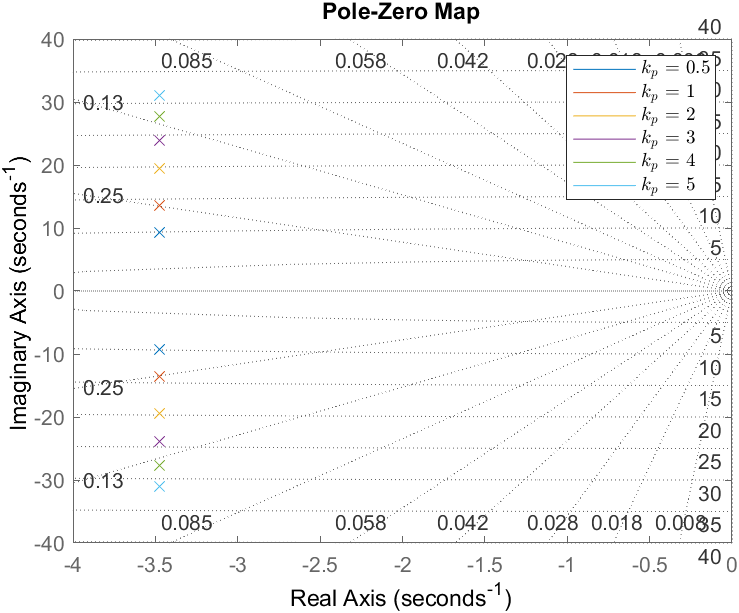
\includegraphics[width=0.94\textwidth]{exp1_pole}
    \caption{\label{fig:exp1_pole}Closed-Loop Pole Positions}
\end{figure}

% You should analyse the relationship between the predicted steady-state errors due to disturbances, and the measured errors. You should comment on any discrepancies and relate them to observations that you have made in earlier labs.
From the pre-lab we get that $\left|e_{ss}\right| = \frac{\tau_d}{k_p}$. The theoretical values of $\left|e_{ss}\right|$ for $\tau_d = 0.1745$ and a $k_p$ of 0.5, 1, 2, 3, 4, and 5 are 20, 10, 5, 3.33, 2.5, and 2 degrees, respectively. As we can see, our measured steady-state error values from Table \ref{table:exp1_measurements} are very close to the theoretical values for a $k_p \geq 2$. For $k_p = 0.5$ and $k_p = 1$ there are pretty large discrepancies between the measured and theoretical values, but this is to be expected because from Lab 2, we observed the non-linear effects in the system's step response with small (0.5, 1) values of $k_p$.

\section{Experiment: Proportional Controller Design}
% calculations
To determine the values for $k_p$ that would meet the design specifications (produce an underdamped response with maximum overshoot of 50\%, 55\%, 60\%, and 65\%), we used the expression from the lab document to estimate the percent overshoot of an underdamped system. The expression was rearranged to solve for $k_p$ in Equation~\ref{eq:calc_kp}. The calculations to determine the values that would meet the specifications were done in MATLAB, with the MATLAB code shown in Listing~\ref{listing:exp2_calc_kp}. The values of $A$ and $\tau_m$ were the average of their determined values from time-domain and frequency-domain analysis in lab 2.
\begin{equation} \label{eq:calc_kp}
\begin{aligned}[b]
    P.O. &= 100\exp\left( -\frac{\pi}{\sqrt{4k_pA\tau_m-1}} \right) \\
    \ln\left(\frac{P.O.}{100}\right) &= -\frac{\pi}{\sqrt{4k_pA\tau_m-1}} \\
    \sqrt{4k_pA\tau_m-1} &= \frac{-\pi}{\ln\left(\frac{P.O.}{100}\right)} \\
    4k_pA\tau_m - 1 &= \left(\frac{-\pi}{\ln\left(\frac{P.O.}{100}\right)}\right)^2 \\
    4k_pA\tau_m &= \left(\frac{-\pi}{\ln\left(\frac{P.O.}{100}\right)}\right)^2 + 1 \\
    k_p &= \left( \left(\frac{-\pi}{\ln\left(\frac{P.O.}{100}\right)}\right)^2 + 1 \right) \ / \ 4A\tau_m
\end{aligned}
\end{equation}
\lstinputlisting[style=Matlab-editor, caption={Calculating $k_p$ to meet specifications}, label={listing:exp2_calc_kp}, lastline=6]{exp_calculations.m}

% measurement procedure goes here
The procedure for measuring the peak overshoot, steady-state error and settling time was identical to the procedure followed in the previous experiment. The peak overshoot and settling time were measured with no step disturbance ($\tau_d = 0$), while the steady-state error was measured with a step disturbance ($\tau_d = 0.1745$). The measurements are presented in Table \ref{table:exp2_measurements}. The figures for the step response plots are shown in Appendix \ref{appendix:exp2fig}.

\begin{table}[h!]
\centering
\begin{tabular}{|c|c|c|c|c|} \hline
    $k_p$ & 1.3314 & 1.7685 & 2.3395 & 3.3489 \\ \hline
    theoretical peak overshoot (\%) & 50 & 55 & 60 & 65 \\ \hline
    peak overshoot (\%) & 41.0 & 50.4 & 59.8 & 69.9 \\ \hline
    theoretical steady-state error (deg) & 7.51 & 5.65 & 4.17 & 2.99 \\ \hline
    steady-state error (deg) & 6.68 & 7.03 & 3.34 & 2.11 \\ \hline
    settling time (sec) & 0.53 & 0.51 & 0.58 & 0.70 \\ \hline 
\end{tabular}
\caption{\label{table:exp2_measurements}Measurements for Experiment 2}
\end{table}

%observations go here
Moving from our first value of $k_p$ to our second, we observed some unusual behaviour where the steady state error increased and the settling time decreased, which is the opposite of what we expected to happen. We re-ran the test multiple times and still achieved the same results every time. This behaviour can be seen in the figures for $k_p = 1.3314$ (Figure~\ref{fig:exp2_kp1.3314}) and $k_p = 1.7685$ (Figure~\ref{fig:exp2_kp1.7685}). Apart from this irregular result at a $k_p$ of 1.7685, the rest of the results followed the expected trend of peak overshoot increasing, steady state error decreasing and settling time increasing, as we increased our $k_p$.

% explain why results are more accurate for higher overshoot
We also observed that the theoretical values for the peak overshoot and the steady-state error were closer to the measured results for higher values of $k_p$ (and higher theoretical peak overshoot). We believe that the non-linear effects in the system are more prevalent at lower values of $k_p$, which could cause these discrepancies to appear. The expressions used to derive the appropriate value of $k_p$ to meet the design requirements were also estimations for a moderately underdamped closed loop system. It is is likely that the estimations are more accurate for the higher values of overshoot that we had.

The closed-loop positions of the system are shown in Figure~\ref{fig:exp2_pole}. We should expect the same behaviour as the previous experiment, which is largely what we measure in this experiment (except for the unexpected measured behaviour between $k_p = 1.3314$ and $k_p = 1.7685$).

\begin{figure}[h]
    \centering
    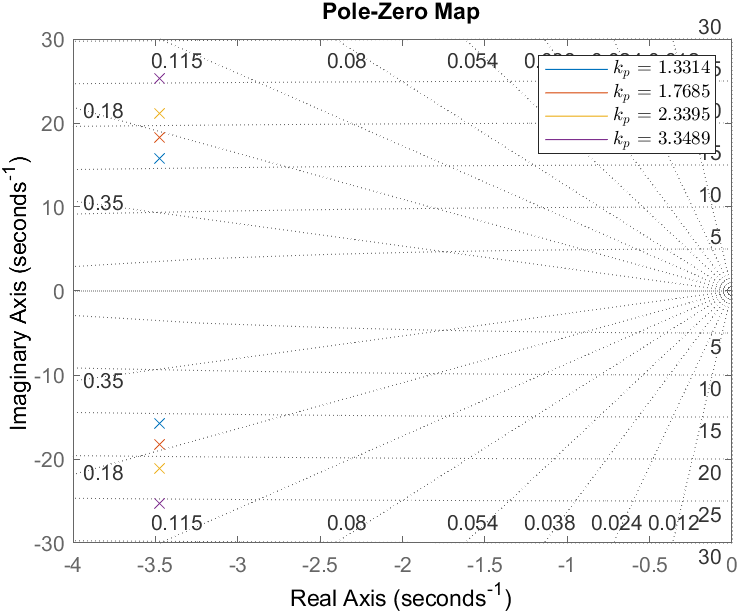
\includegraphics[width=0.94\textwidth]{exp2_pole}
    \caption{\label{fig:exp2_pole}Closed-Loop Pole Positions}
\end{figure}

\setcounter{section}{5}
\section{Joint Design of Proportional Controller and Velocity Feedback}
There are two design requirements to consider. We know that the magnitude of the steady-state error can be given by the expression $\left| e_{ss} \right| = \frac{\tau_d}{k_p}$. If the steady-state error at $k_p = 1$ is 10 degrees, to reduce the steady-state by a factor of 5 (to 2 degrees), we need to increase $k_p$ by a factor of 5. Therefore the design requirement for the magnitude of the steady-state error can be met by any $k_p > 5$. We can also determine the $\zeta$ value of the system for the target percent overshoot of $10\%$, which is done in Equation~\ref{eq:calc_zeta}
\begin{equation} \label{eq:calc_zeta}
    \zeta = -\frac{\ln\left(\frac{P.O.}{100}\right)}{\sqrt{\pi^2 + \ln^2\left(\frac{P.O.}{100}\right)}}
\end{equation}
We can rearrange the expression relating $\zeta$, $k_p$, and $k_v$ to solve for $k_v$, and determine the minimum value of $k_v$ to meet the percent overshoot requirement. This is done in Equation~\ref{eq:calc_kv}
\begin{equation} \label{eq:calc_kv}
\begin{aligned}[b]
    \zeta &= \frac{1+k_vA}{2\sqrt{k_pA\tau_m}} \\
    k_v &= \frac{2\zeta\sqrt{k_pA\tau_m}-1}{A} 
\end{aligned}
\end{equation}
The MATLAB code to determine the minimum values of $k_v$ for various acceptable $k_p$ is shown in Listing~\ref{listing:exp3_calc_kv}.
\lstinputlisting[style=Matlab-editor, caption={Calculating $k_v$ to meet specifications}, label={listing:exp3_calc_kv}, firstline=8, firstnumber=8]{exp_calculations.m}

The procedure for measuring the peak overshoot and steady-state error was identical to the procedure followed in the first experiment. The peak overshoot and steady-state time were measured with a step disturbance ($\tau_d = 0.1745$). The measurements are presented in Table \ref{table:exp3_measurements}. The figures for the step response plots are shown in Appendix \ref{appendix:exp3fig}.

\begin{table}[h!]
\centering
\begin{tabular}{|c|c|c|c|} \hline
    $k_p$ & 5 & 6 & 7 \\ \hline
    $k_v$ & 0.1537 & 0.1718 & 0.1884 \\ \hline
    peak overshoot (\%) & 11.70 & 11.33 & 8.25 \\ \hline
    steady-state error (deg) & 2.11 & 1.76 & 1.41 \\ \hline
\end{tabular}
\caption{\label{table:exp3_measurements}Measurements for Experiment 3}
\end{table}

The results are close to what is expected, with values of peak overshoot and steady-state error near or within the design requirements. We can also observe a similar pattern to what has occurred in the previous experiments, where the expected peak overshoot and steady-state error are within the design requirements (expected from our design) for larger values of $k_p$, but slightly outside our expectations for lower values of $k_p$.

The closed-loop positions of the system are shown in Figure~\ref{fig:exp3_pole}. Based on the pole positions, we should not expect a significant difference in the percent overshoot, as the poles all have the same angle with the negative real axis. Our experiments confirm this, as the percent overshoot for all three combinations of $k_p$ and $k_v$ are relatively similar.

\begin{figure}[h]
    \centering
    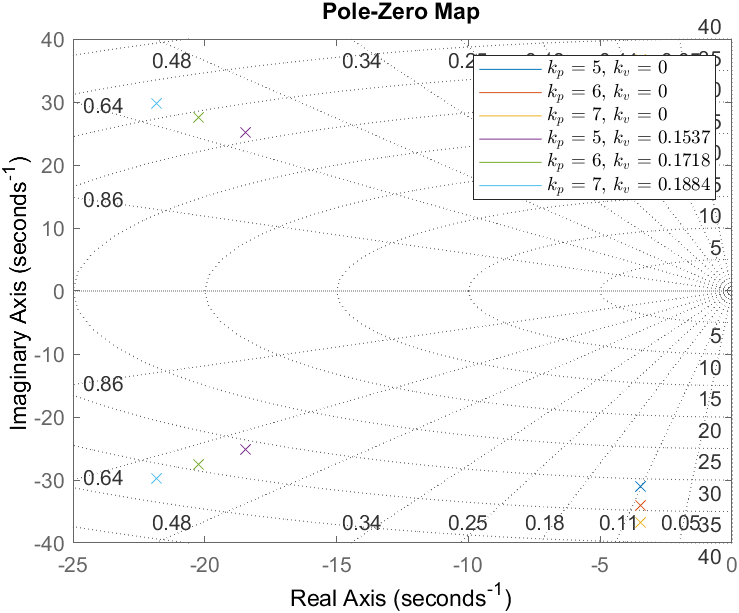
\includegraphics[width=0.94\textwidth]{exp3_pole}
    \caption{\label{fig:exp3_pole}Closed-Loop Pole Positions}
\end{figure}

\section*{Comparison of Proportional Control and Proportional Control with Velocity Feedback}
The system with no velocity feedback requires you to make trade-offs between the overshoot and rise time of the system, as both parameters are affected by changes in $k_p$. The addition of the velocity of feedback allows you to modify the system with more flexibility as you can adjust one parameter without requiring a trade-off in the other.
 
The system with velocity feedback will also have poles that are further out, therefore it will decay much faster. This results in a system with less overshoot, faster rise time, and less settling time. 

\clearpage
\appendix
\section{Experiment 1 Figures} \label{appendix:exp1fig}
\begin{figure}[h]
    \centering
    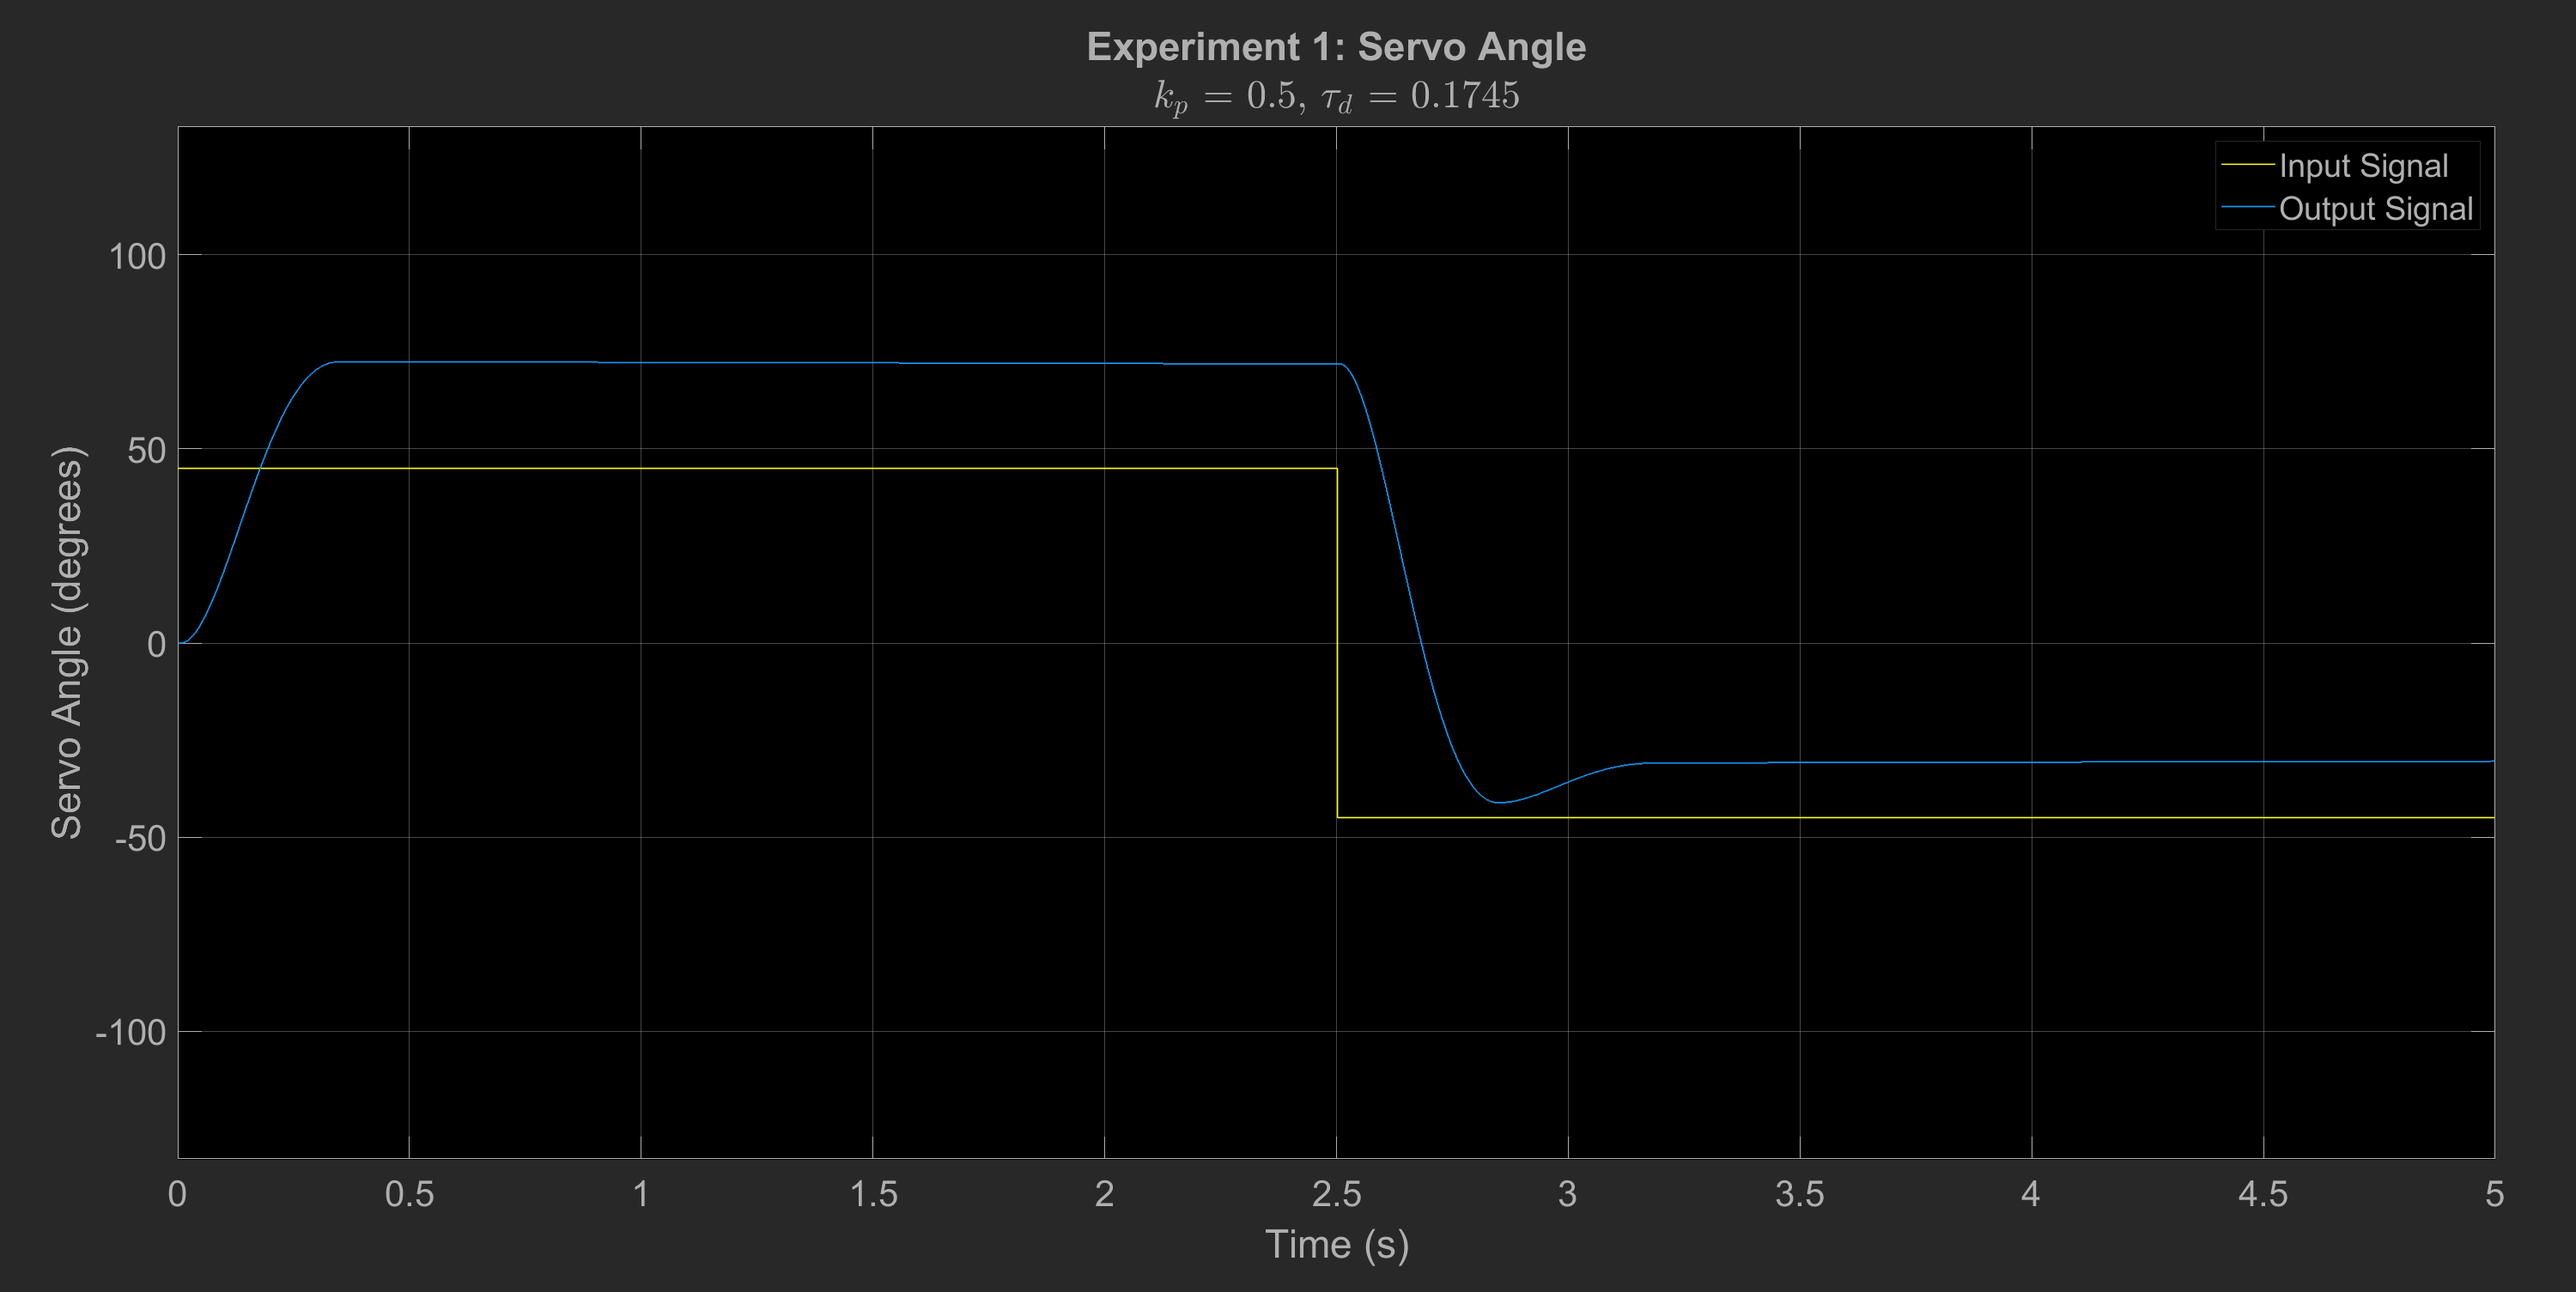
\includegraphics[width=0.91\textwidth]{exp1_kp0.5}
    \caption{Experiment 1: $k_p = 0.5$}
\end{figure}
\begin{figure}[h]
    \centering
    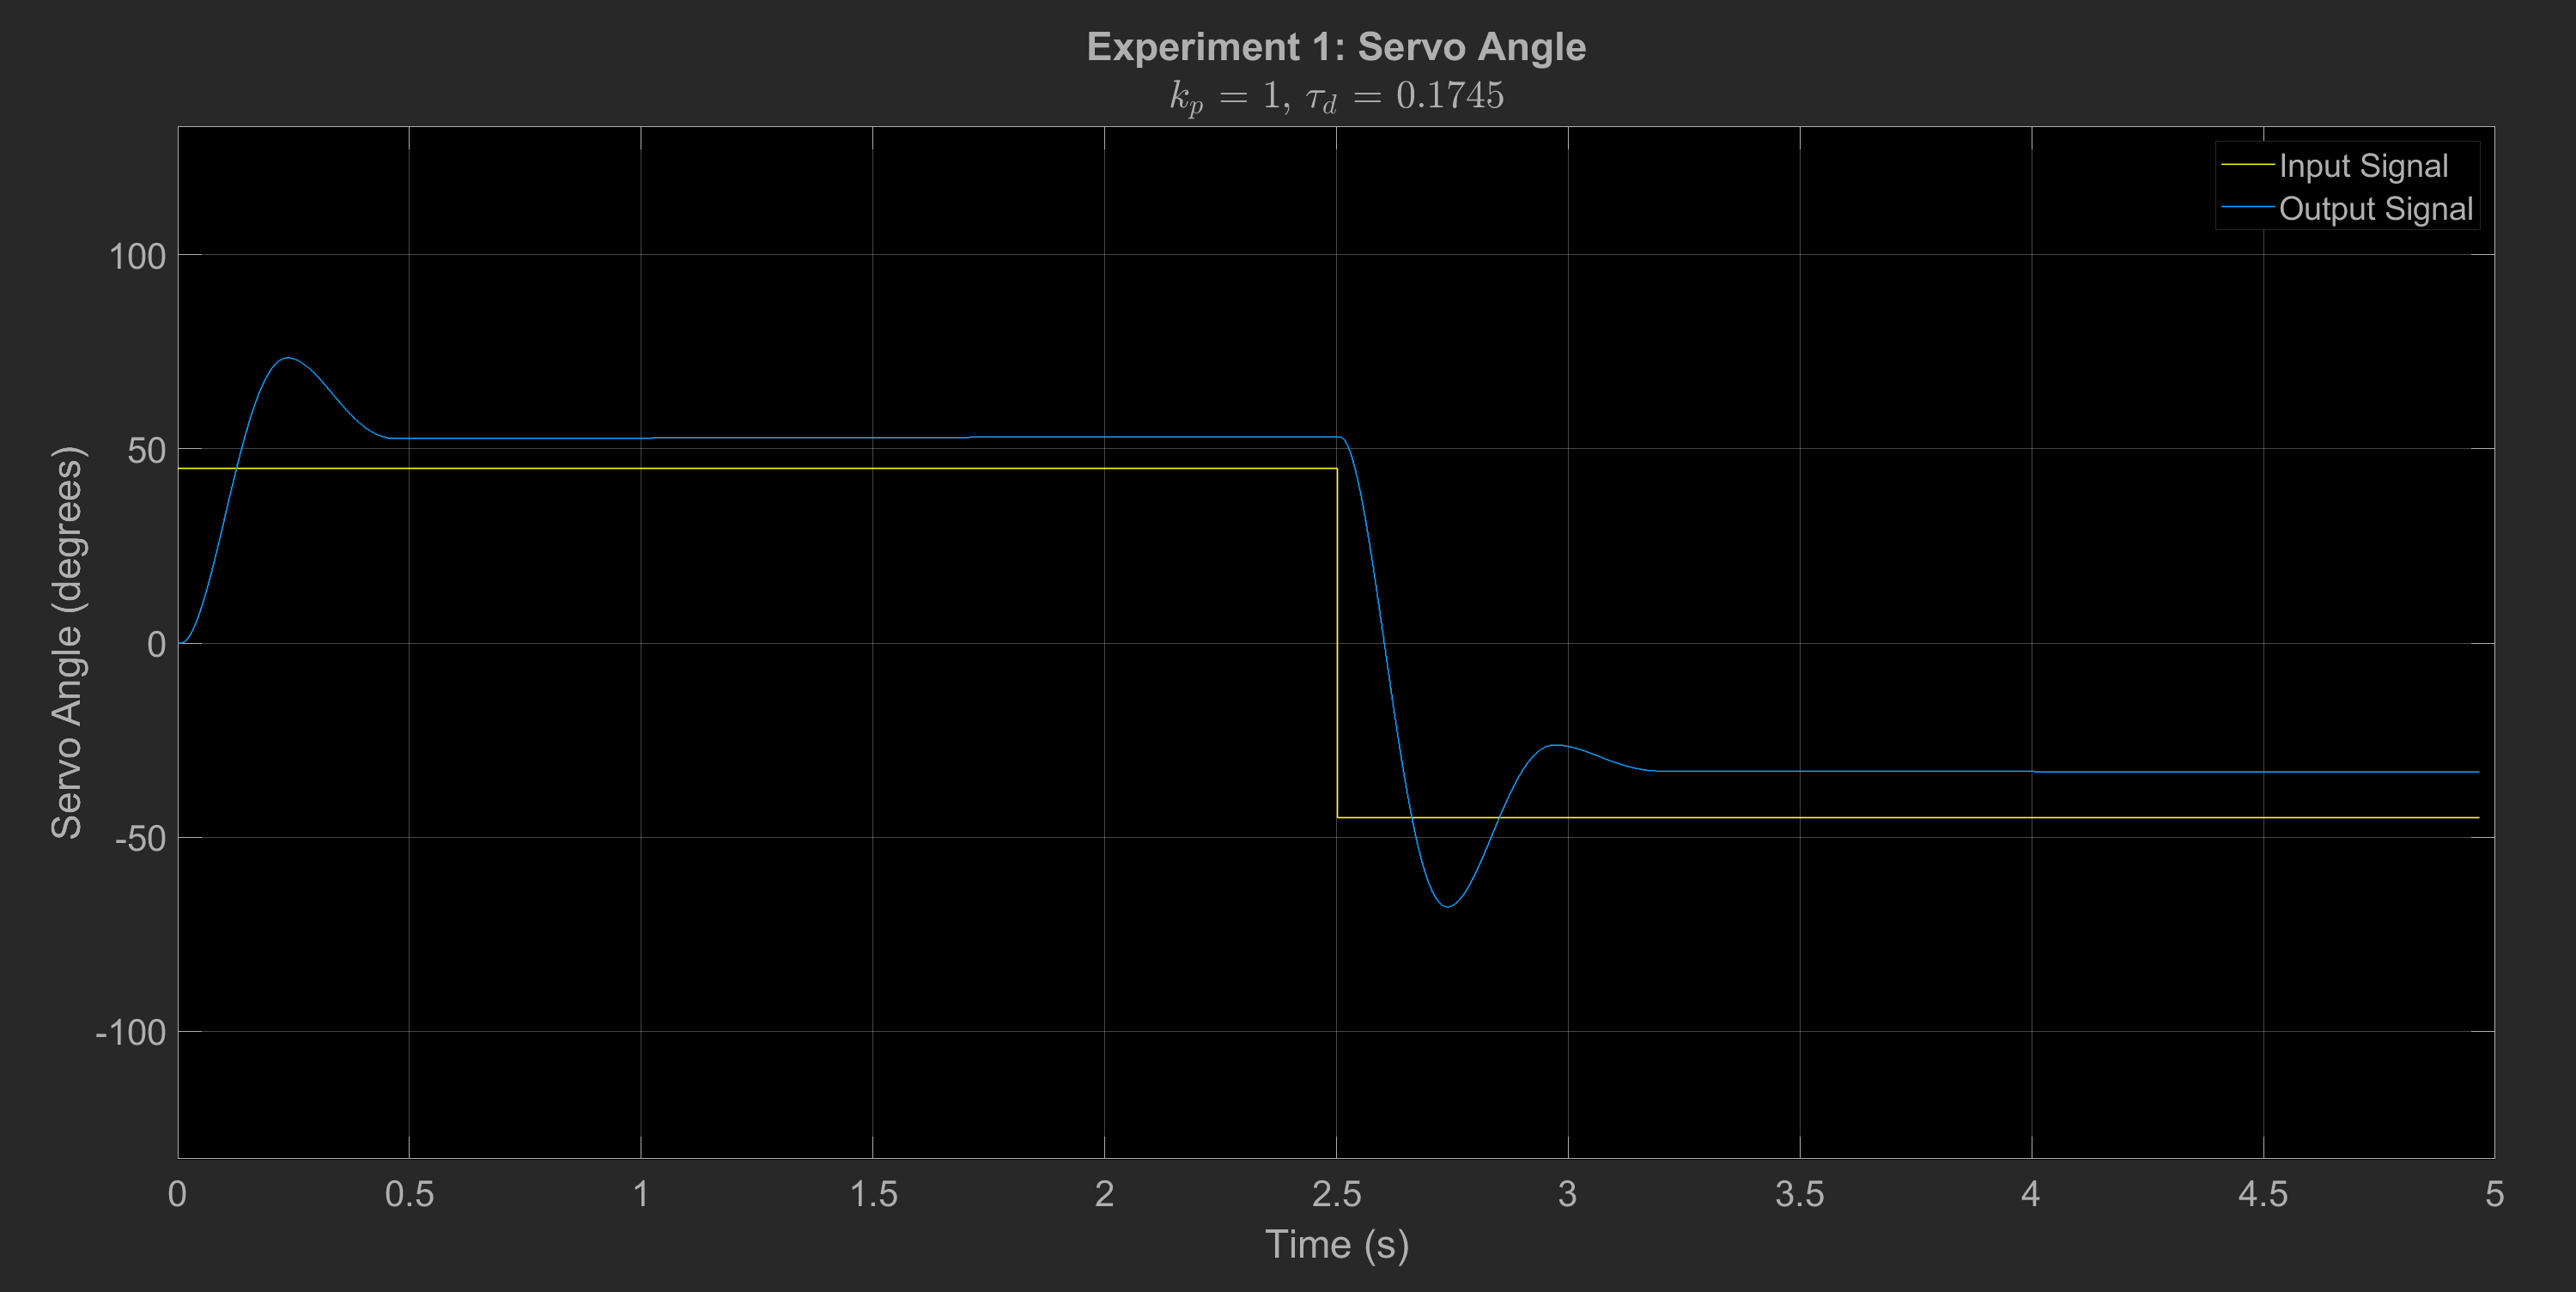
\includegraphics[width=0.91\textwidth]{exp1_kp1}
    \caption{Experiment 1: $k_p = 1$}
\end{figure}
\begin{figure}[h]
    \centering
    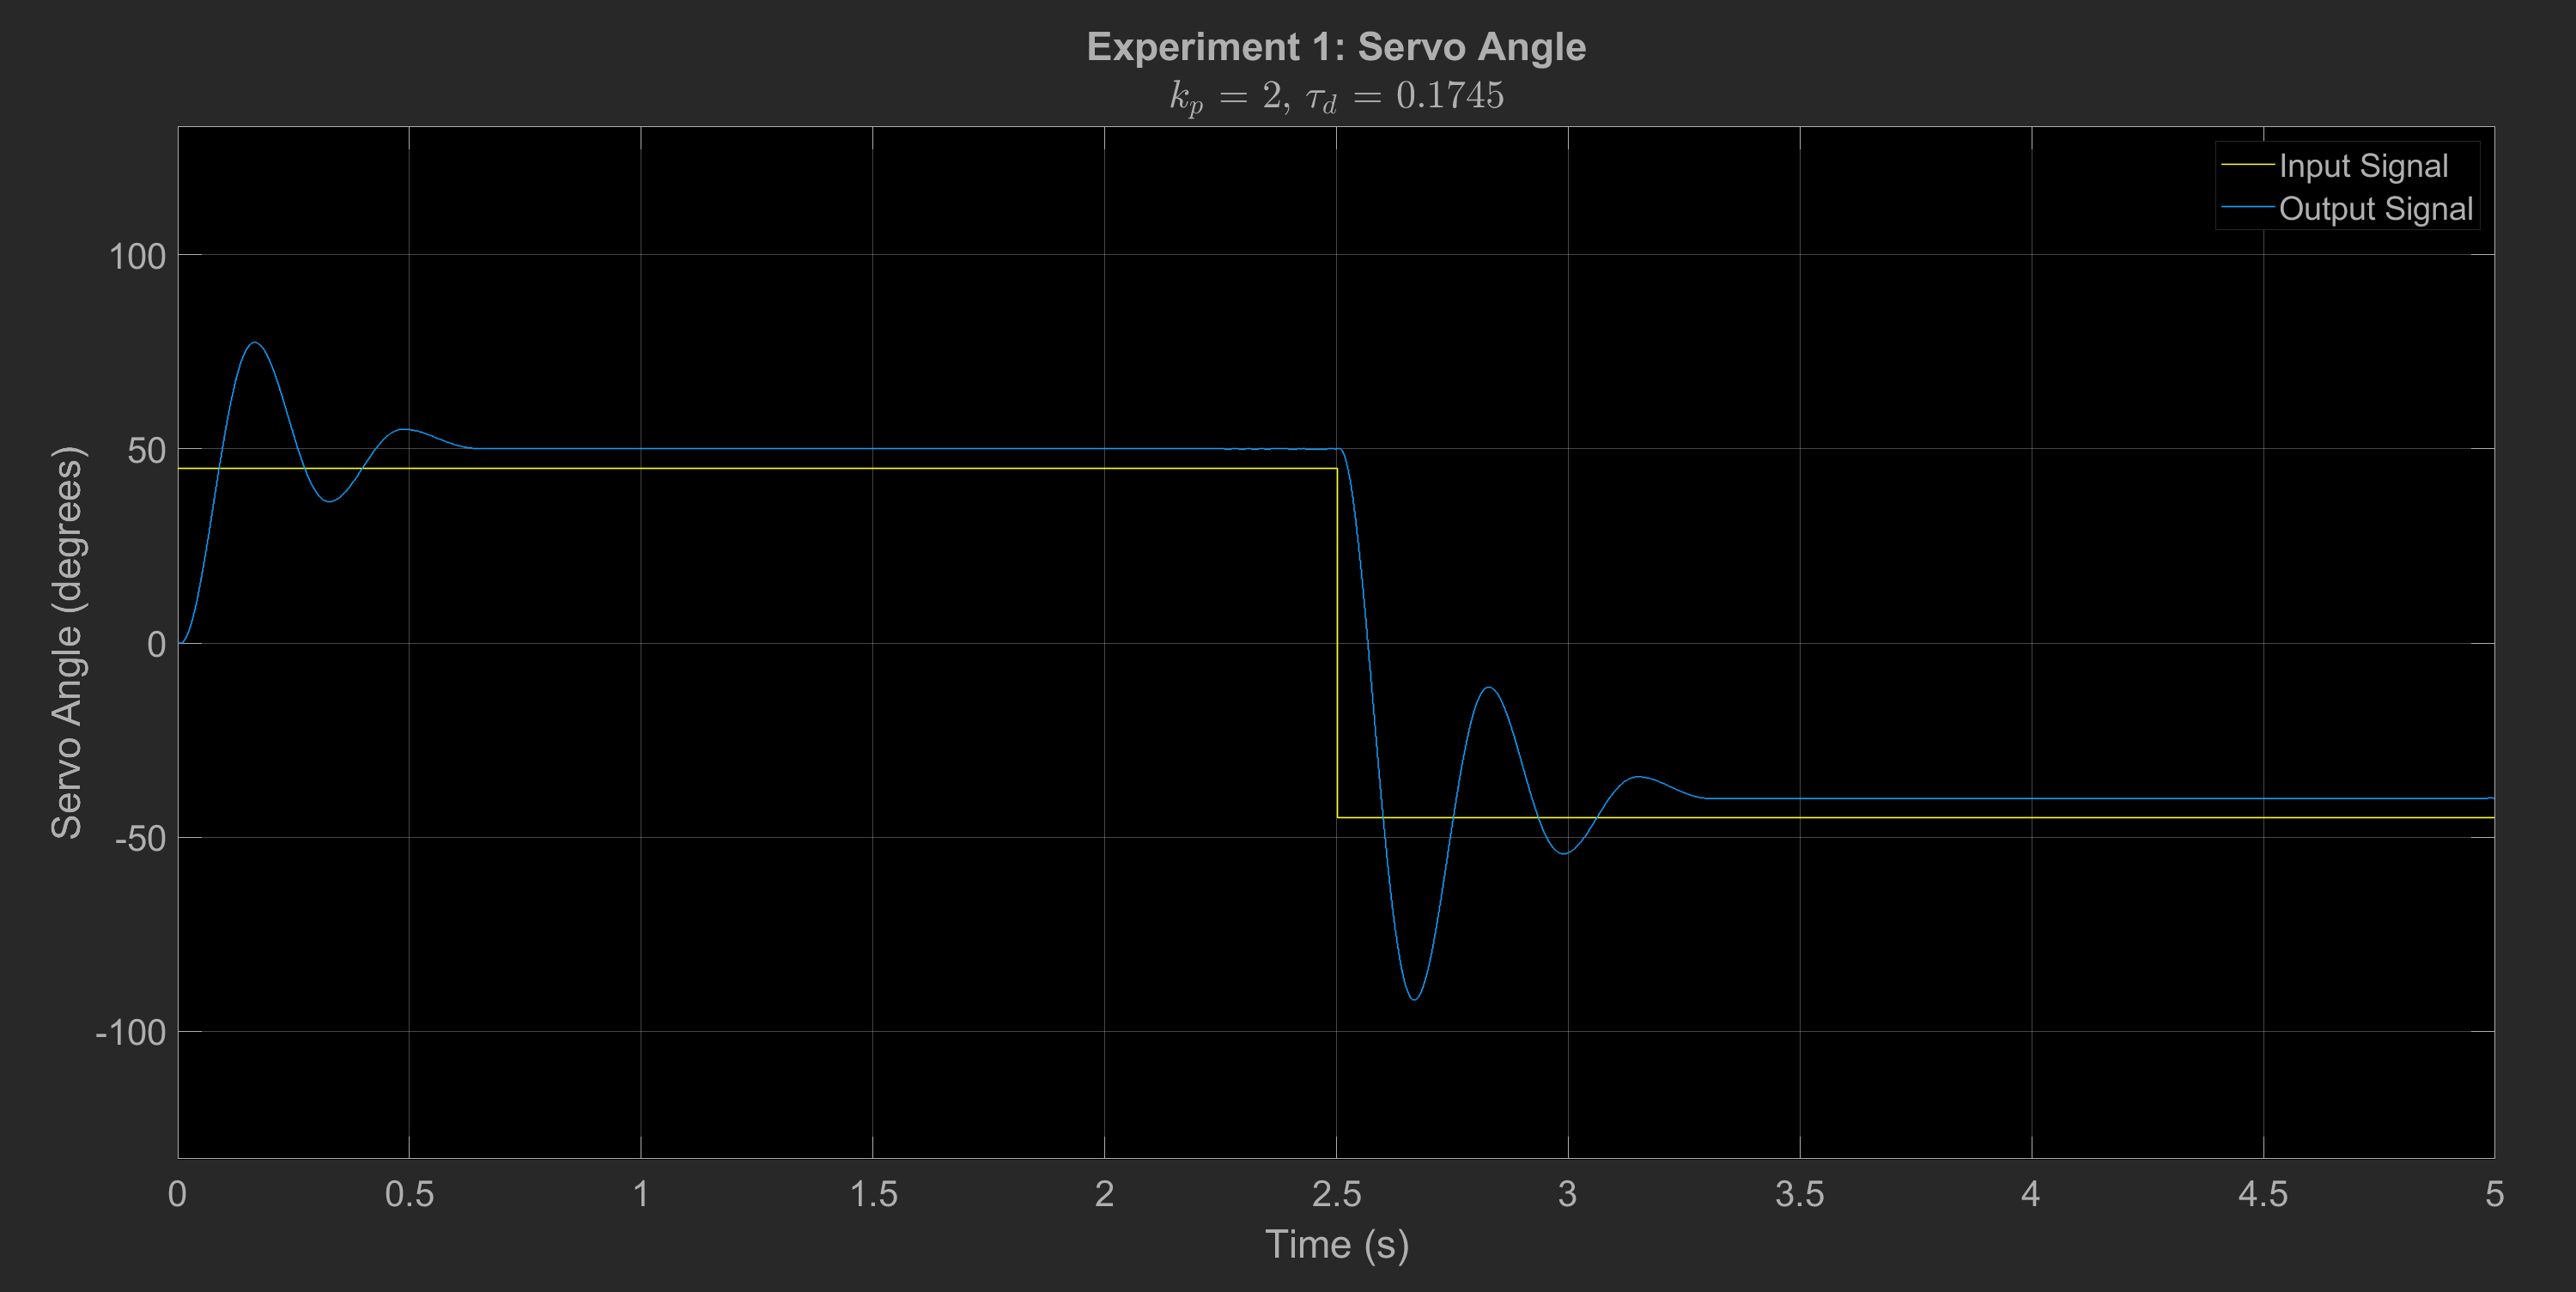
\includegraphics[width=0.91\textwidth]{exp1_kp2}
    \caption{Experiment 1: $k_p = 2$}
\end{figure}
\begin{figure}[h]
    \centering
    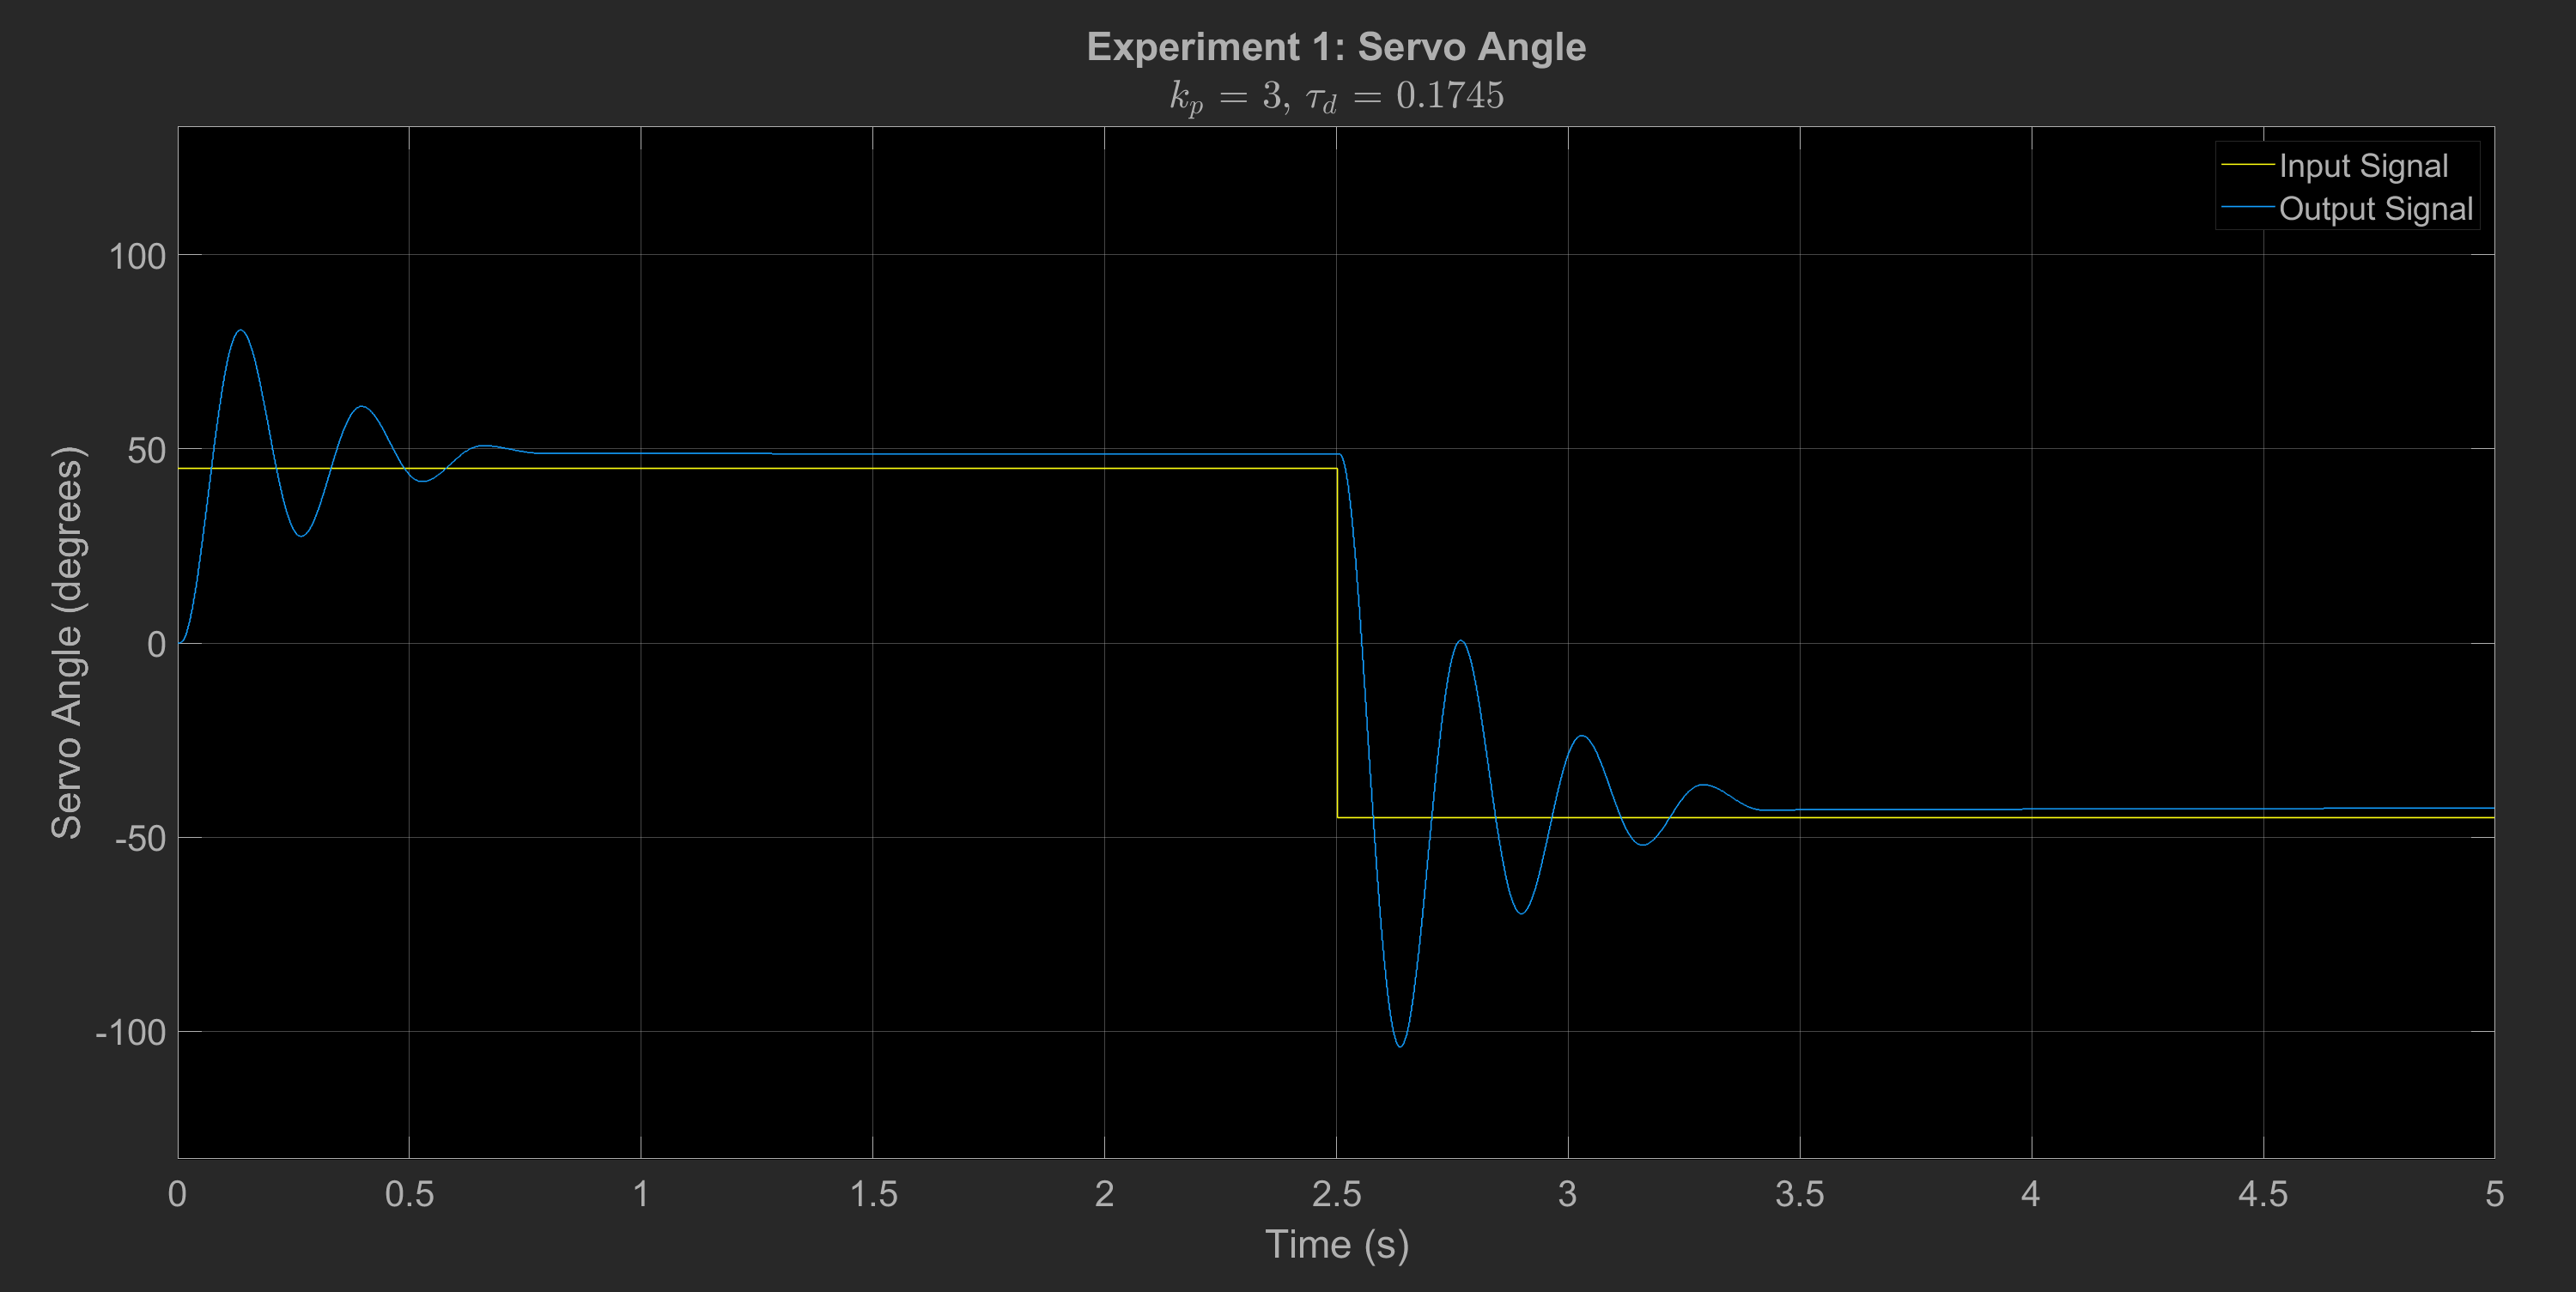
\includegraphics[width=0.91\textwidth]{exp1_kp3}
    \caption{Experiment 1: $k_p = 3$}
\end{figure}
\begin{figure}[h]
    \centering
    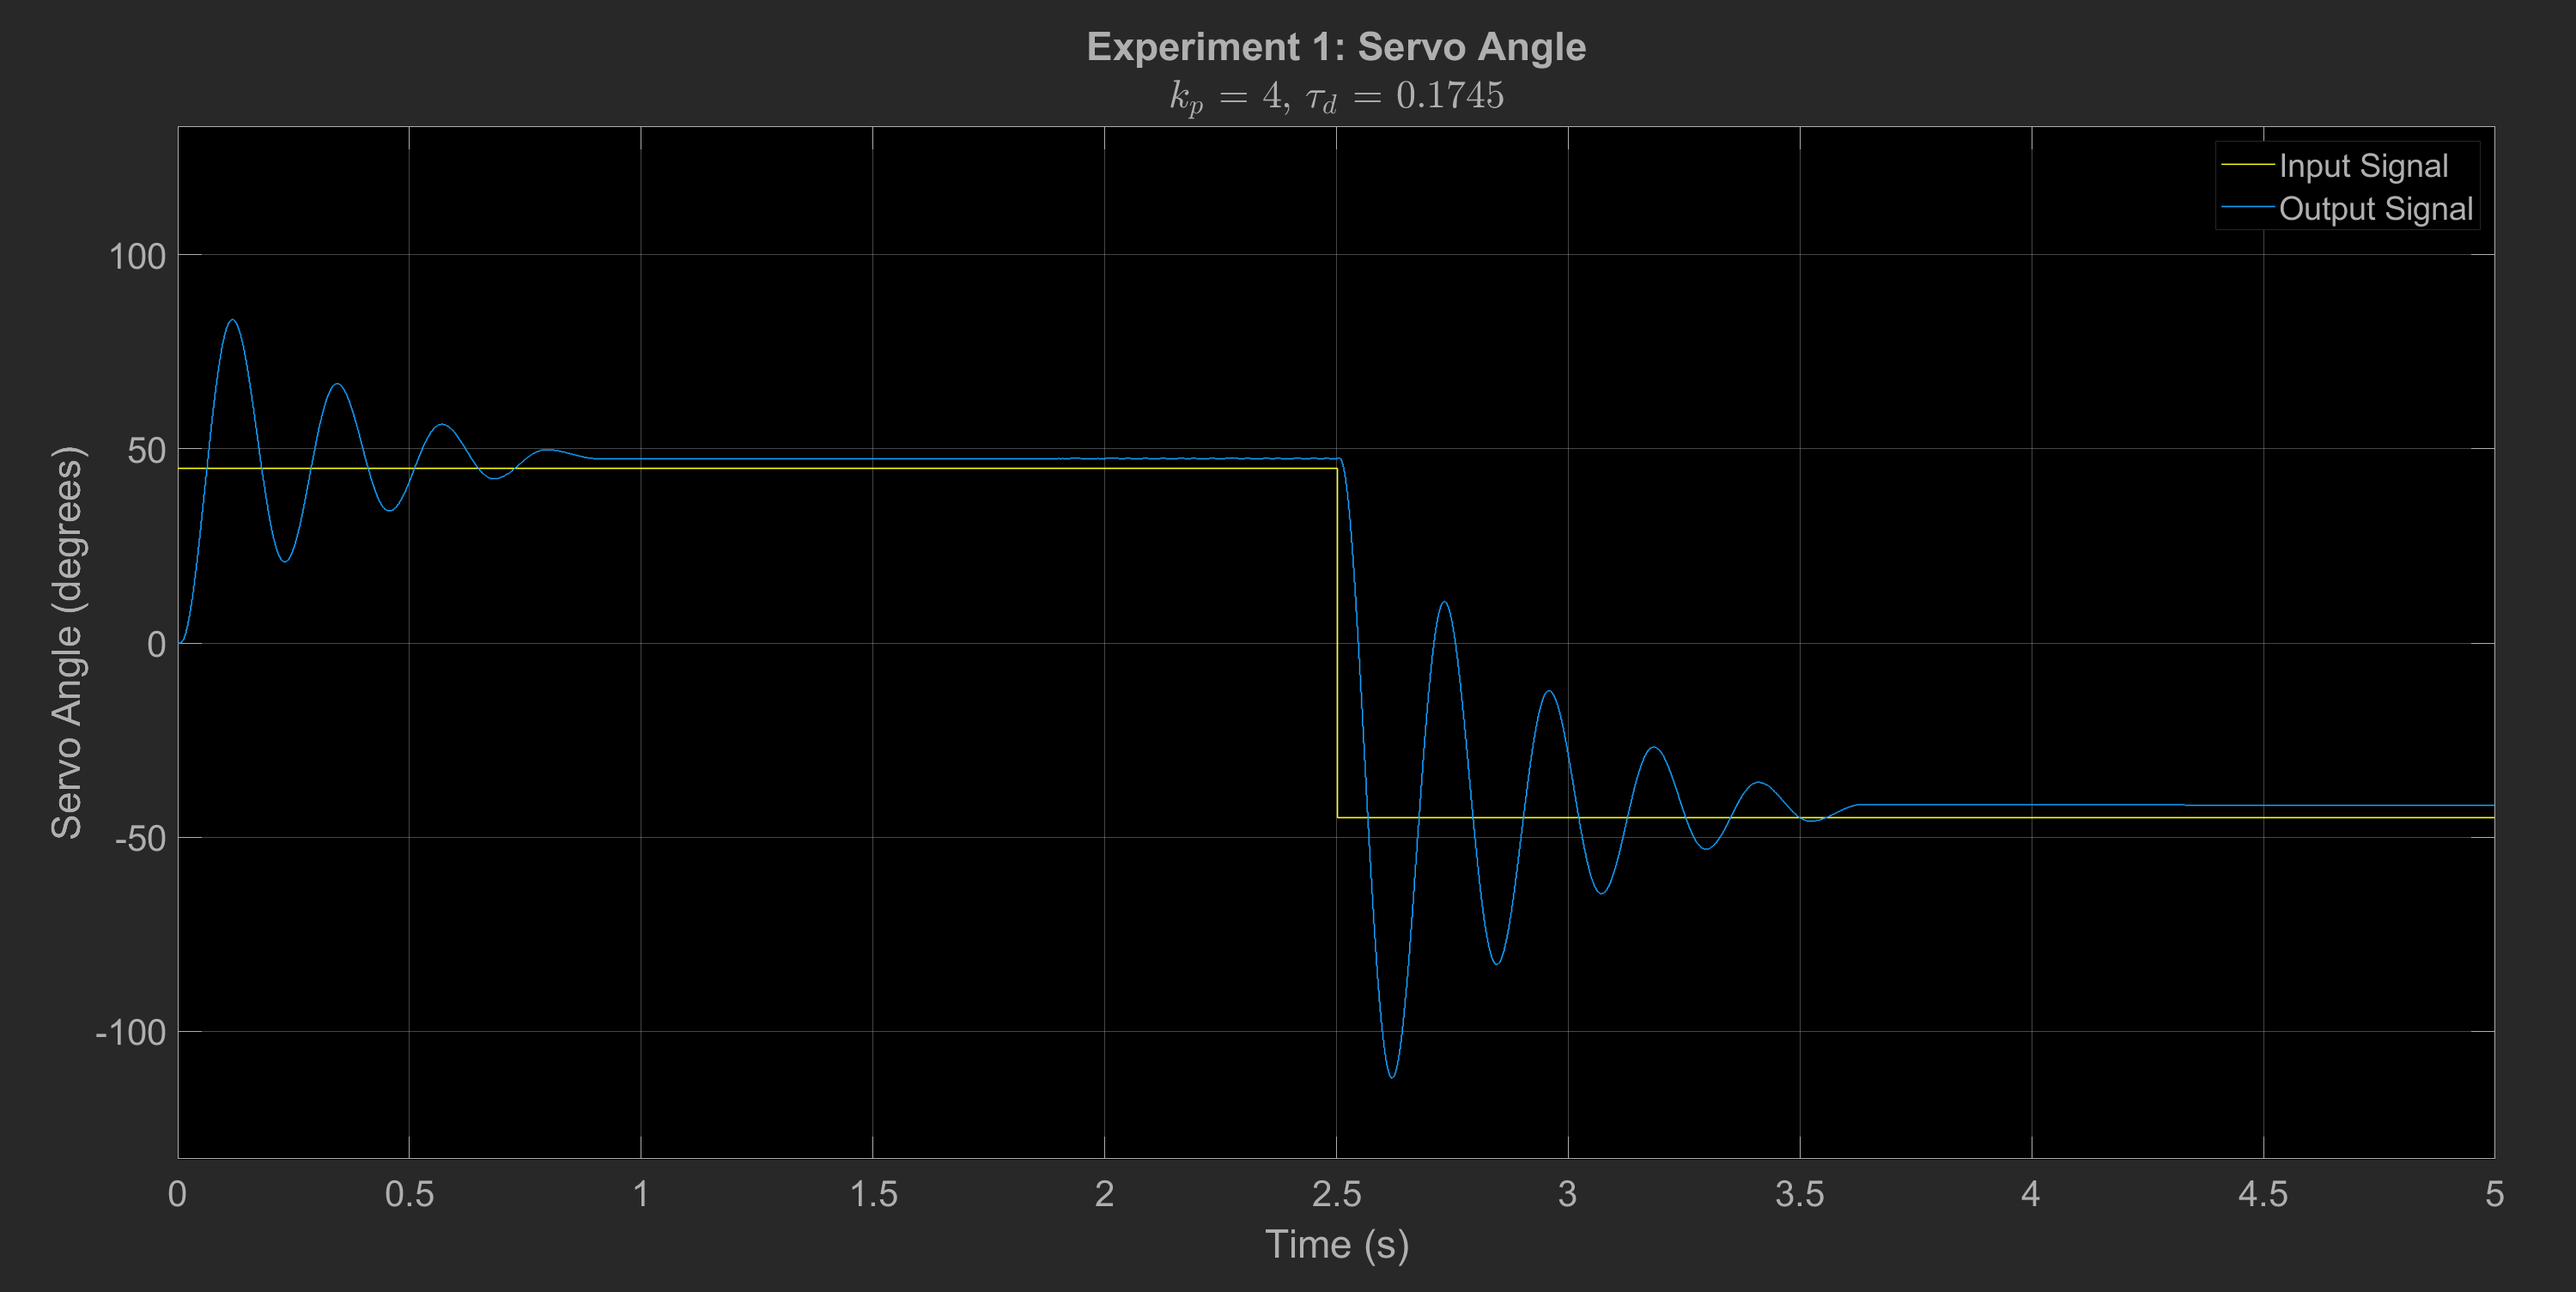
\includegraphics[width=0.91\textwidth]{exp1_kp4}
    \caption{Experiment 1: $k_p = 4$}
\end{figure}
\begin{figure}[h]
    \centering
    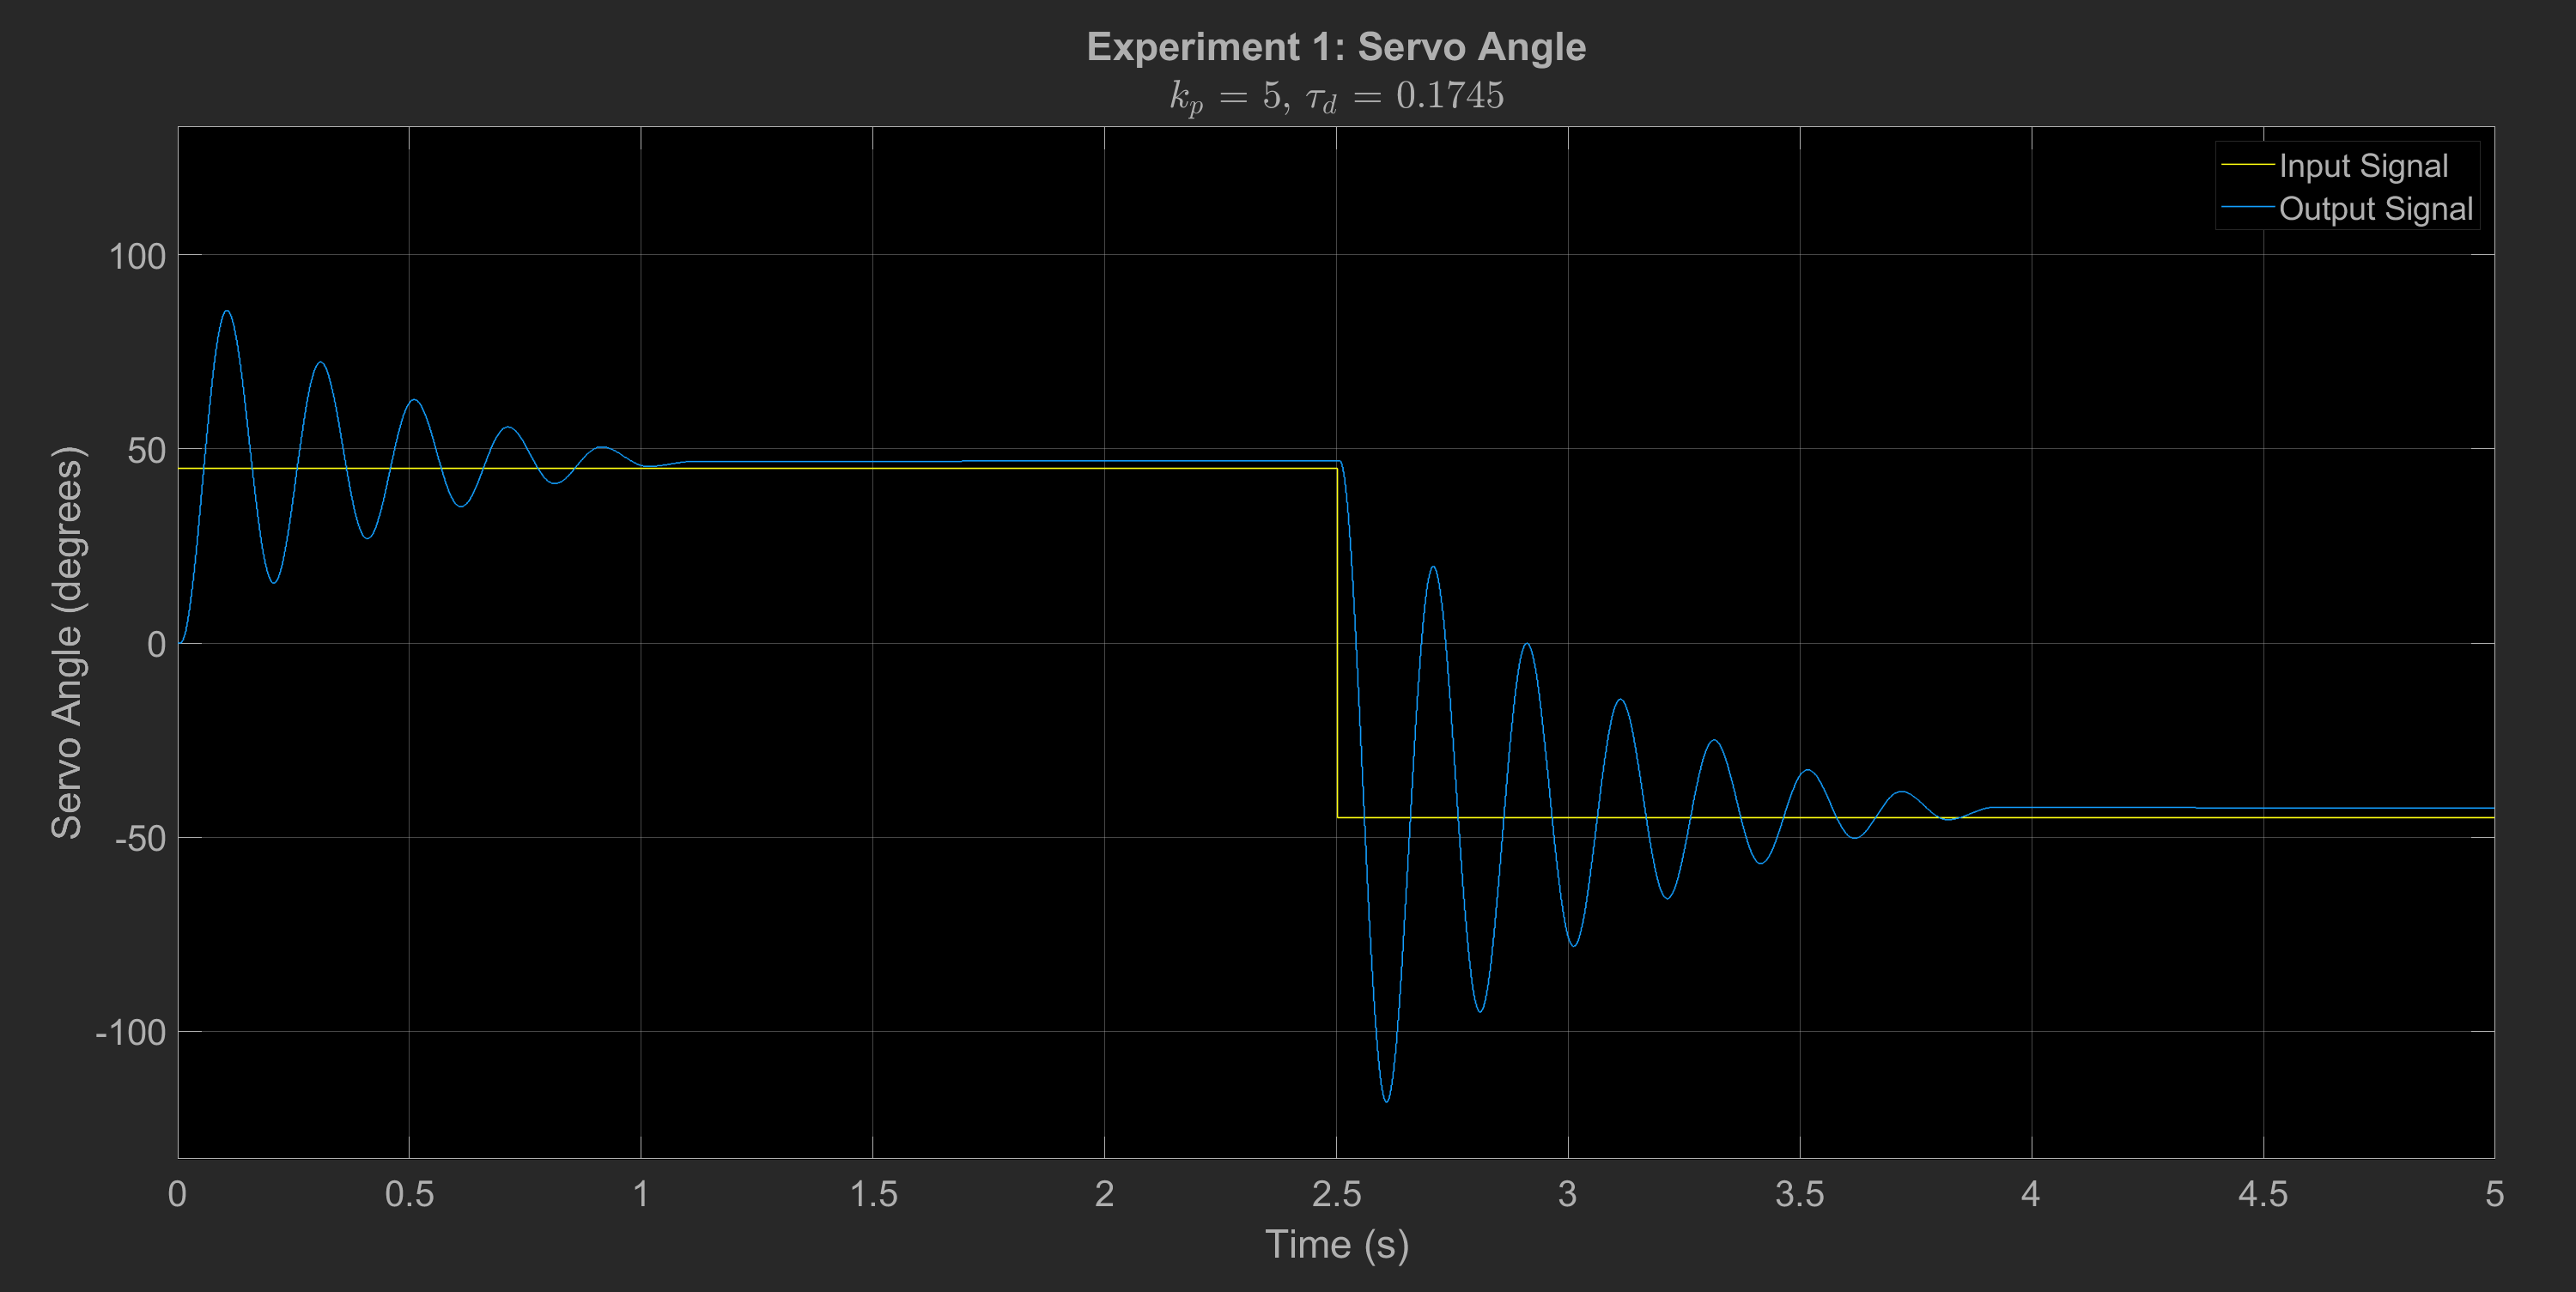
\includegraphics[width=0.91\textwidth]{exp1_kp5}
    \caption{Experiment 1: $k_p = 5$}
\end{figure}

\clearpage
\section{Experiment 2 Figures} \label{appendix:exp2fig}
\begin{figure}[h]
    \centering
    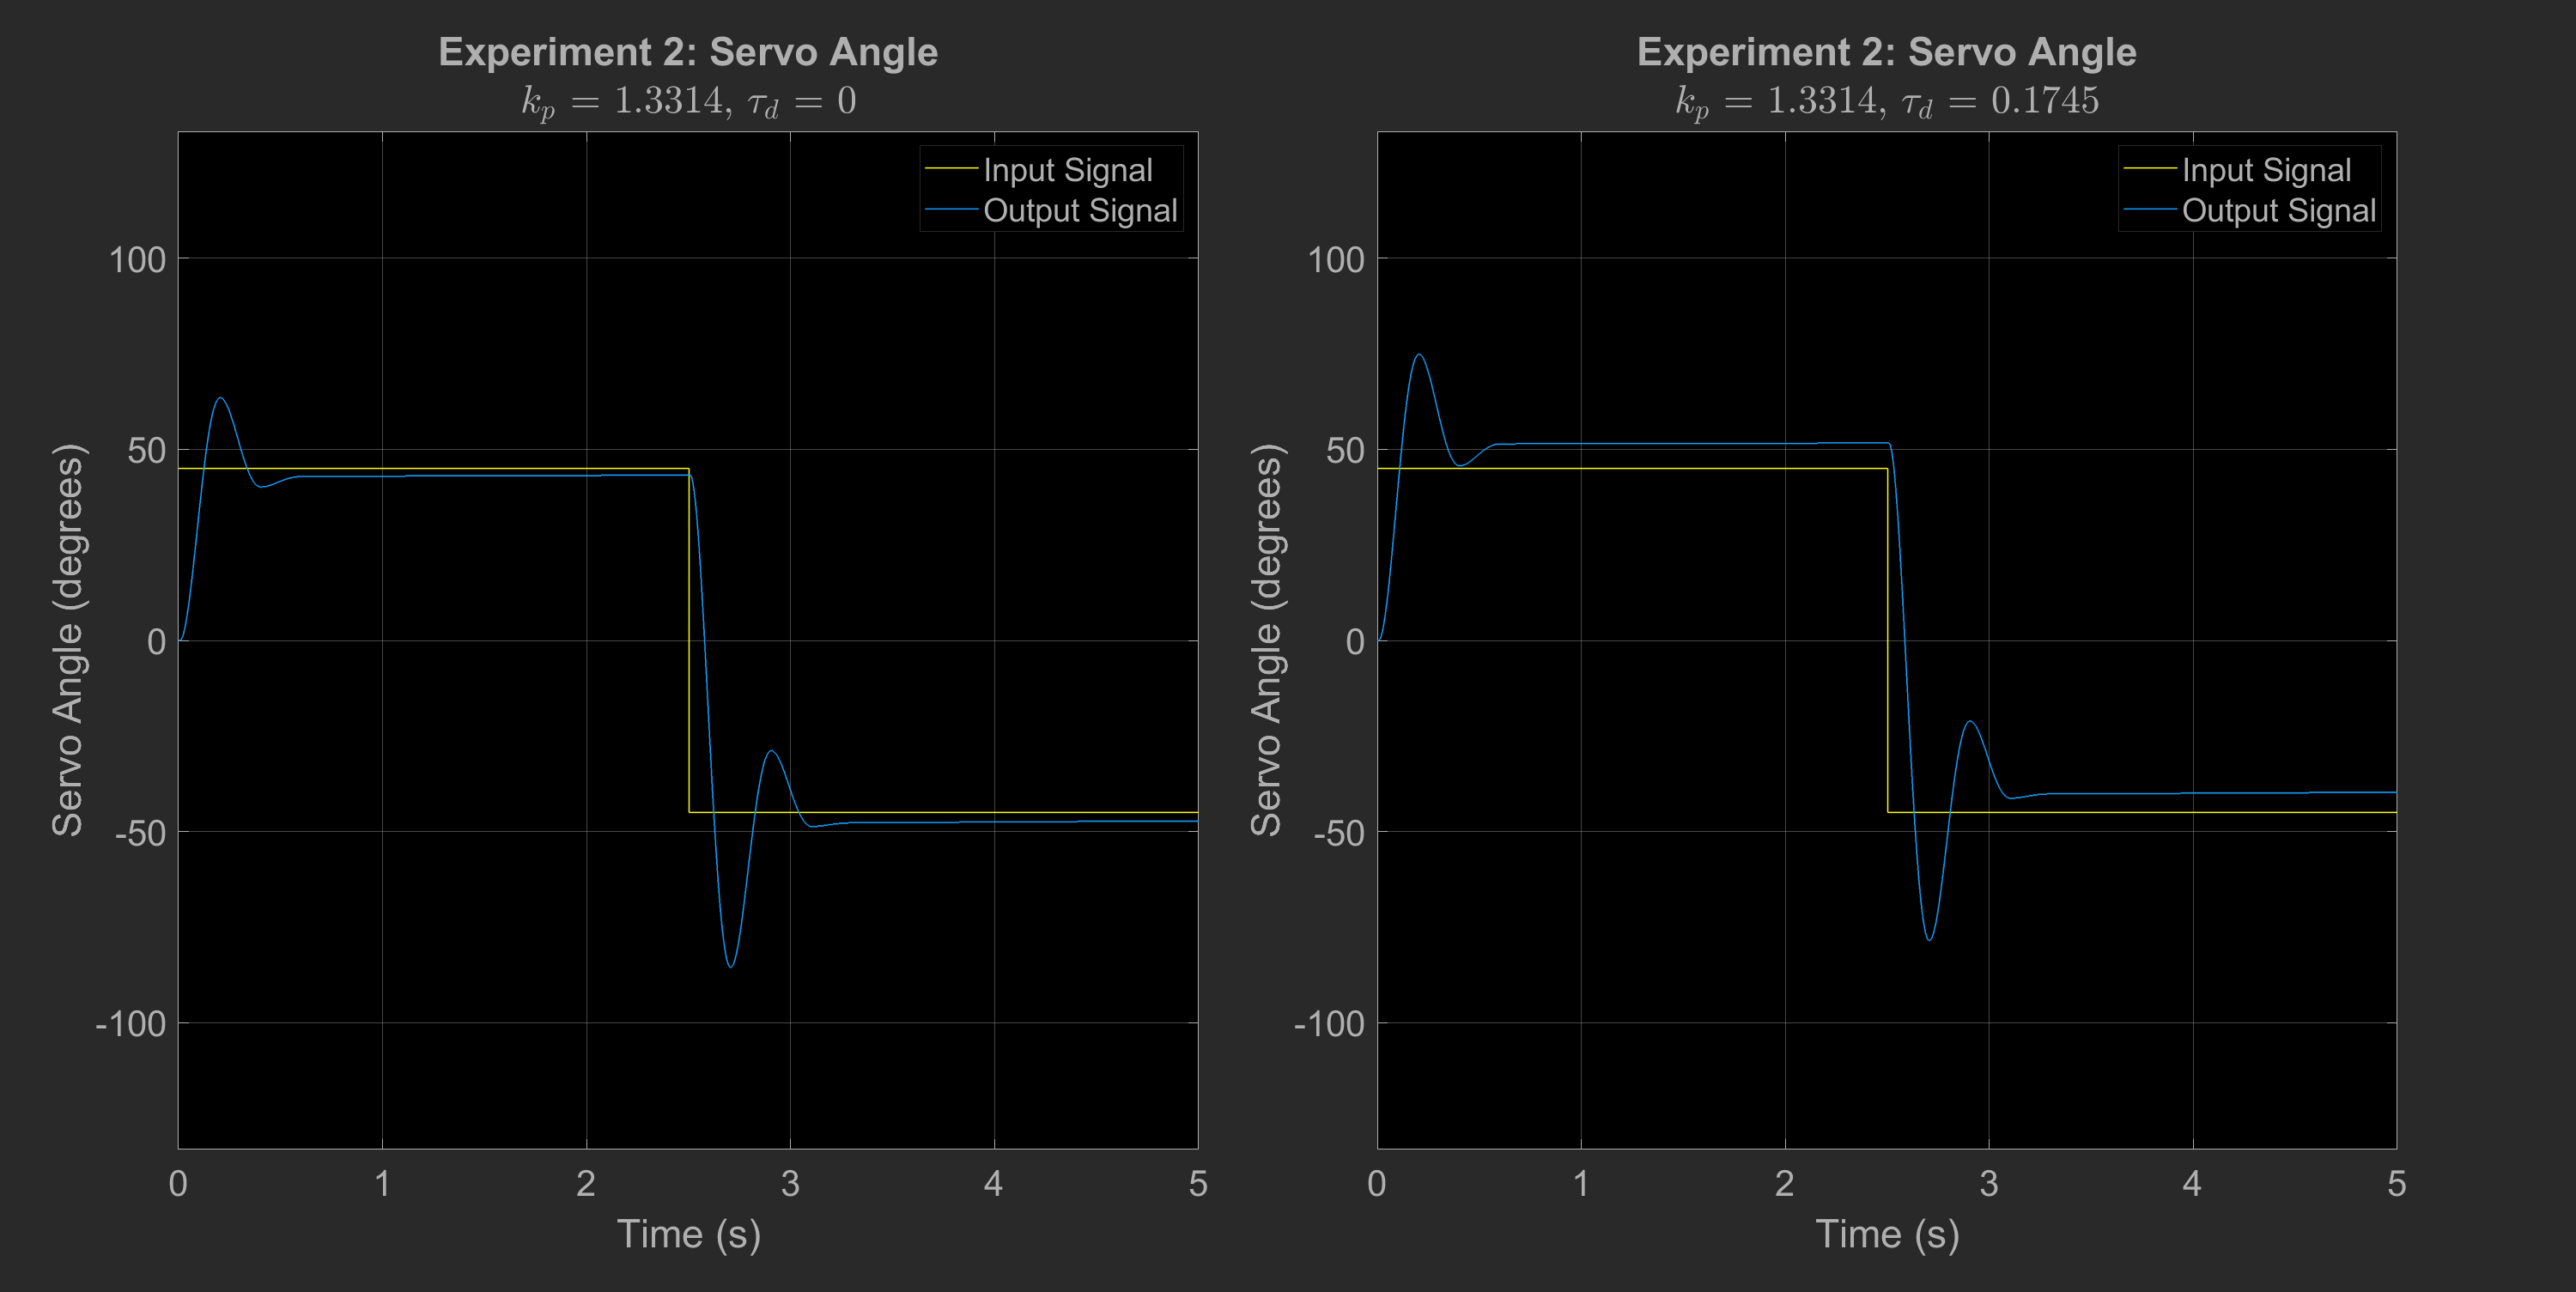
\includegraphics[width=0.91\textwidth]{exp2_kp1.3314}
    \caption{\label{fig:exp2_kp1.3314}Experiment 2: $k_p = 1.3314$}
\end{figure}
\begin{figure}[h]
    \centering
    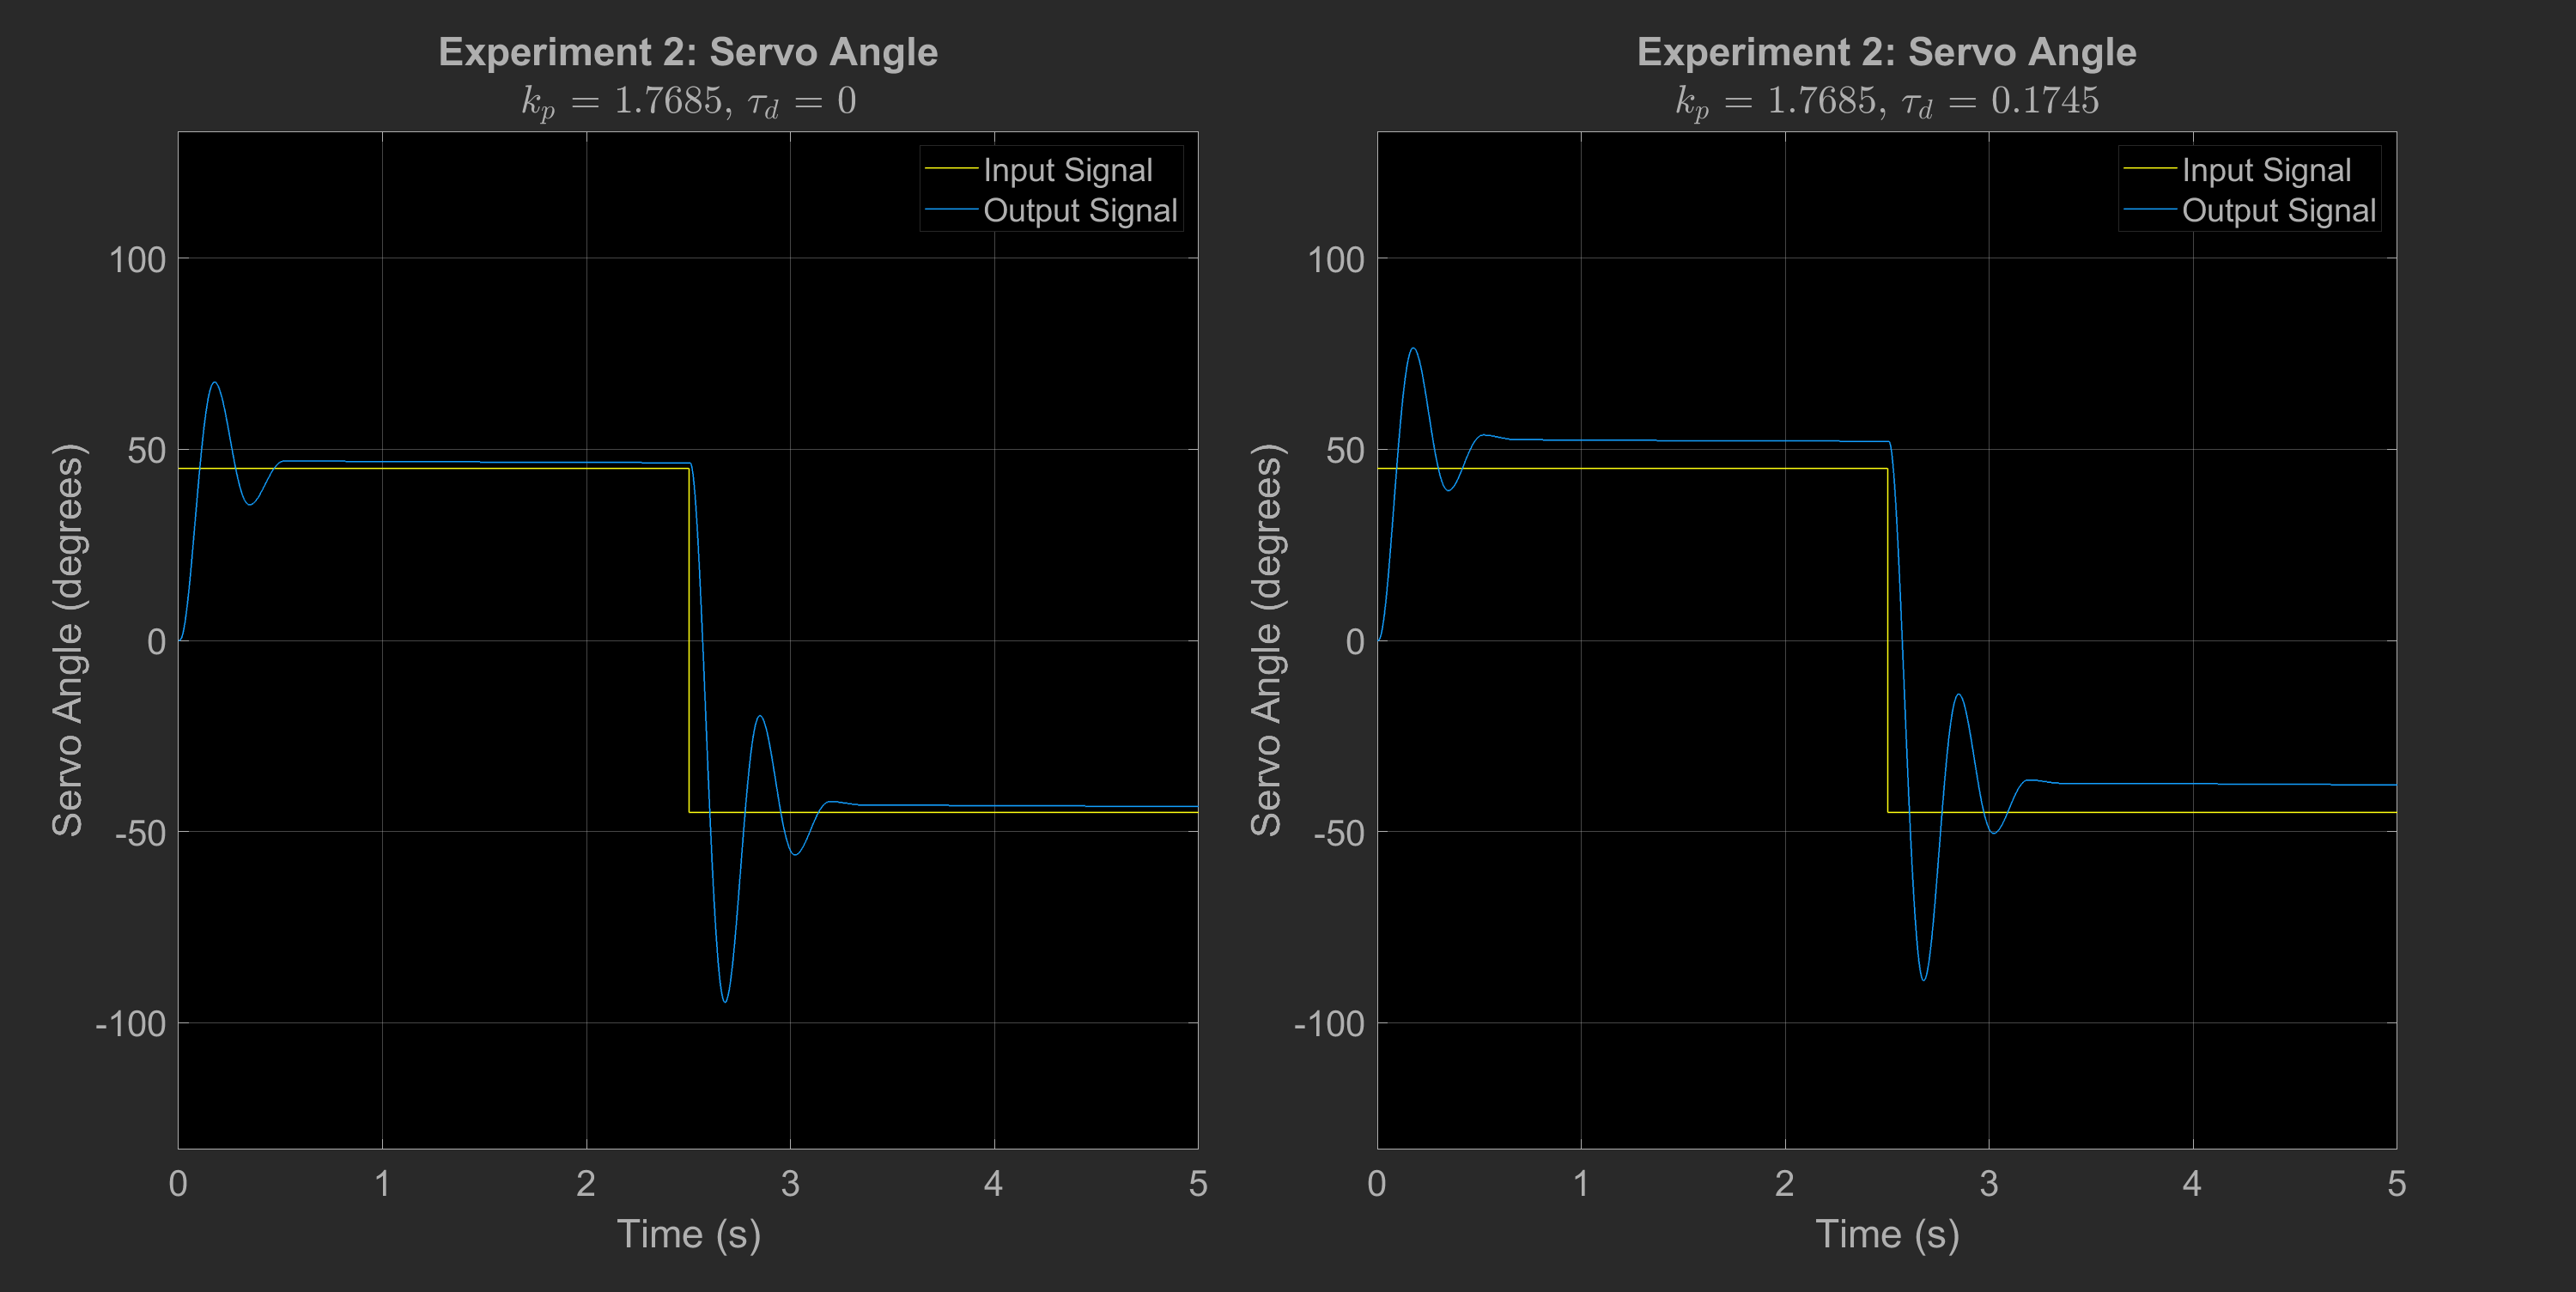
\includegraphics[width=0.91\textwidth]{exp2_kp1.7685}
    \caption{\label{fig:exp2_kp1.7685}Experiment 2: $k_p = 1.7685$}
\end{figure}
\begin{figure}[h]
    \centering
    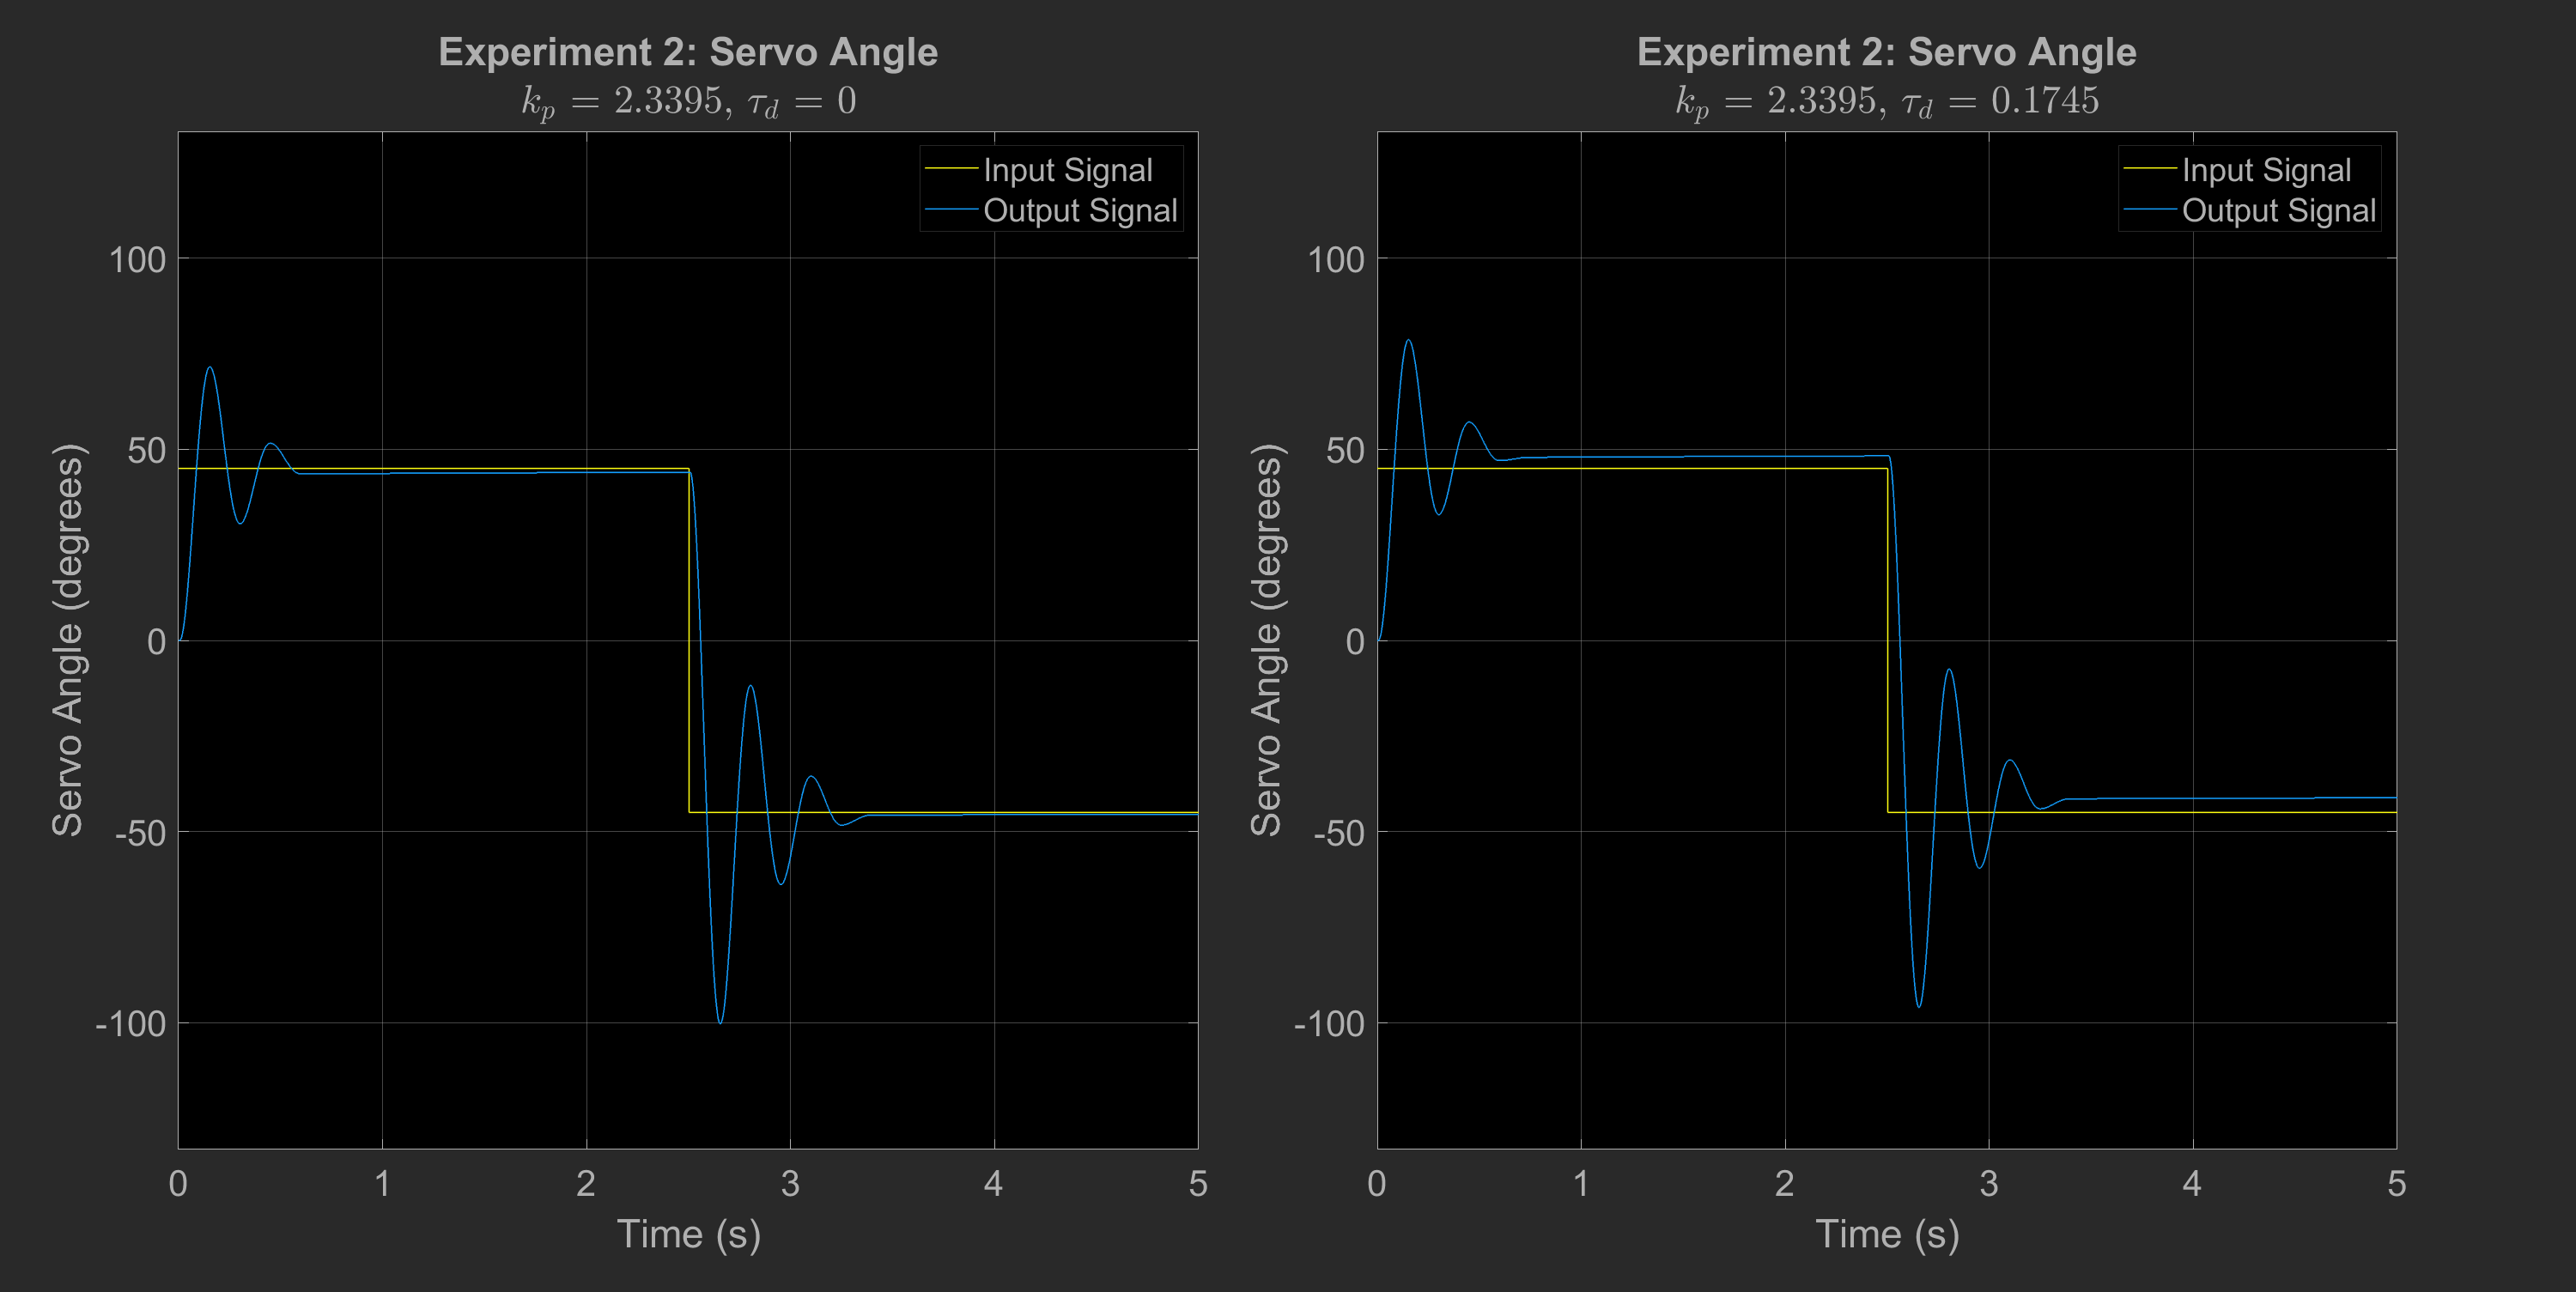
\includegraphics[width=0.91\textwidth]{exp2_kp2.3395}
    \caption{Experiment 2: $k_p = 2.3395$}
\end{figure}
\begin{figure}[h]
    \centering
    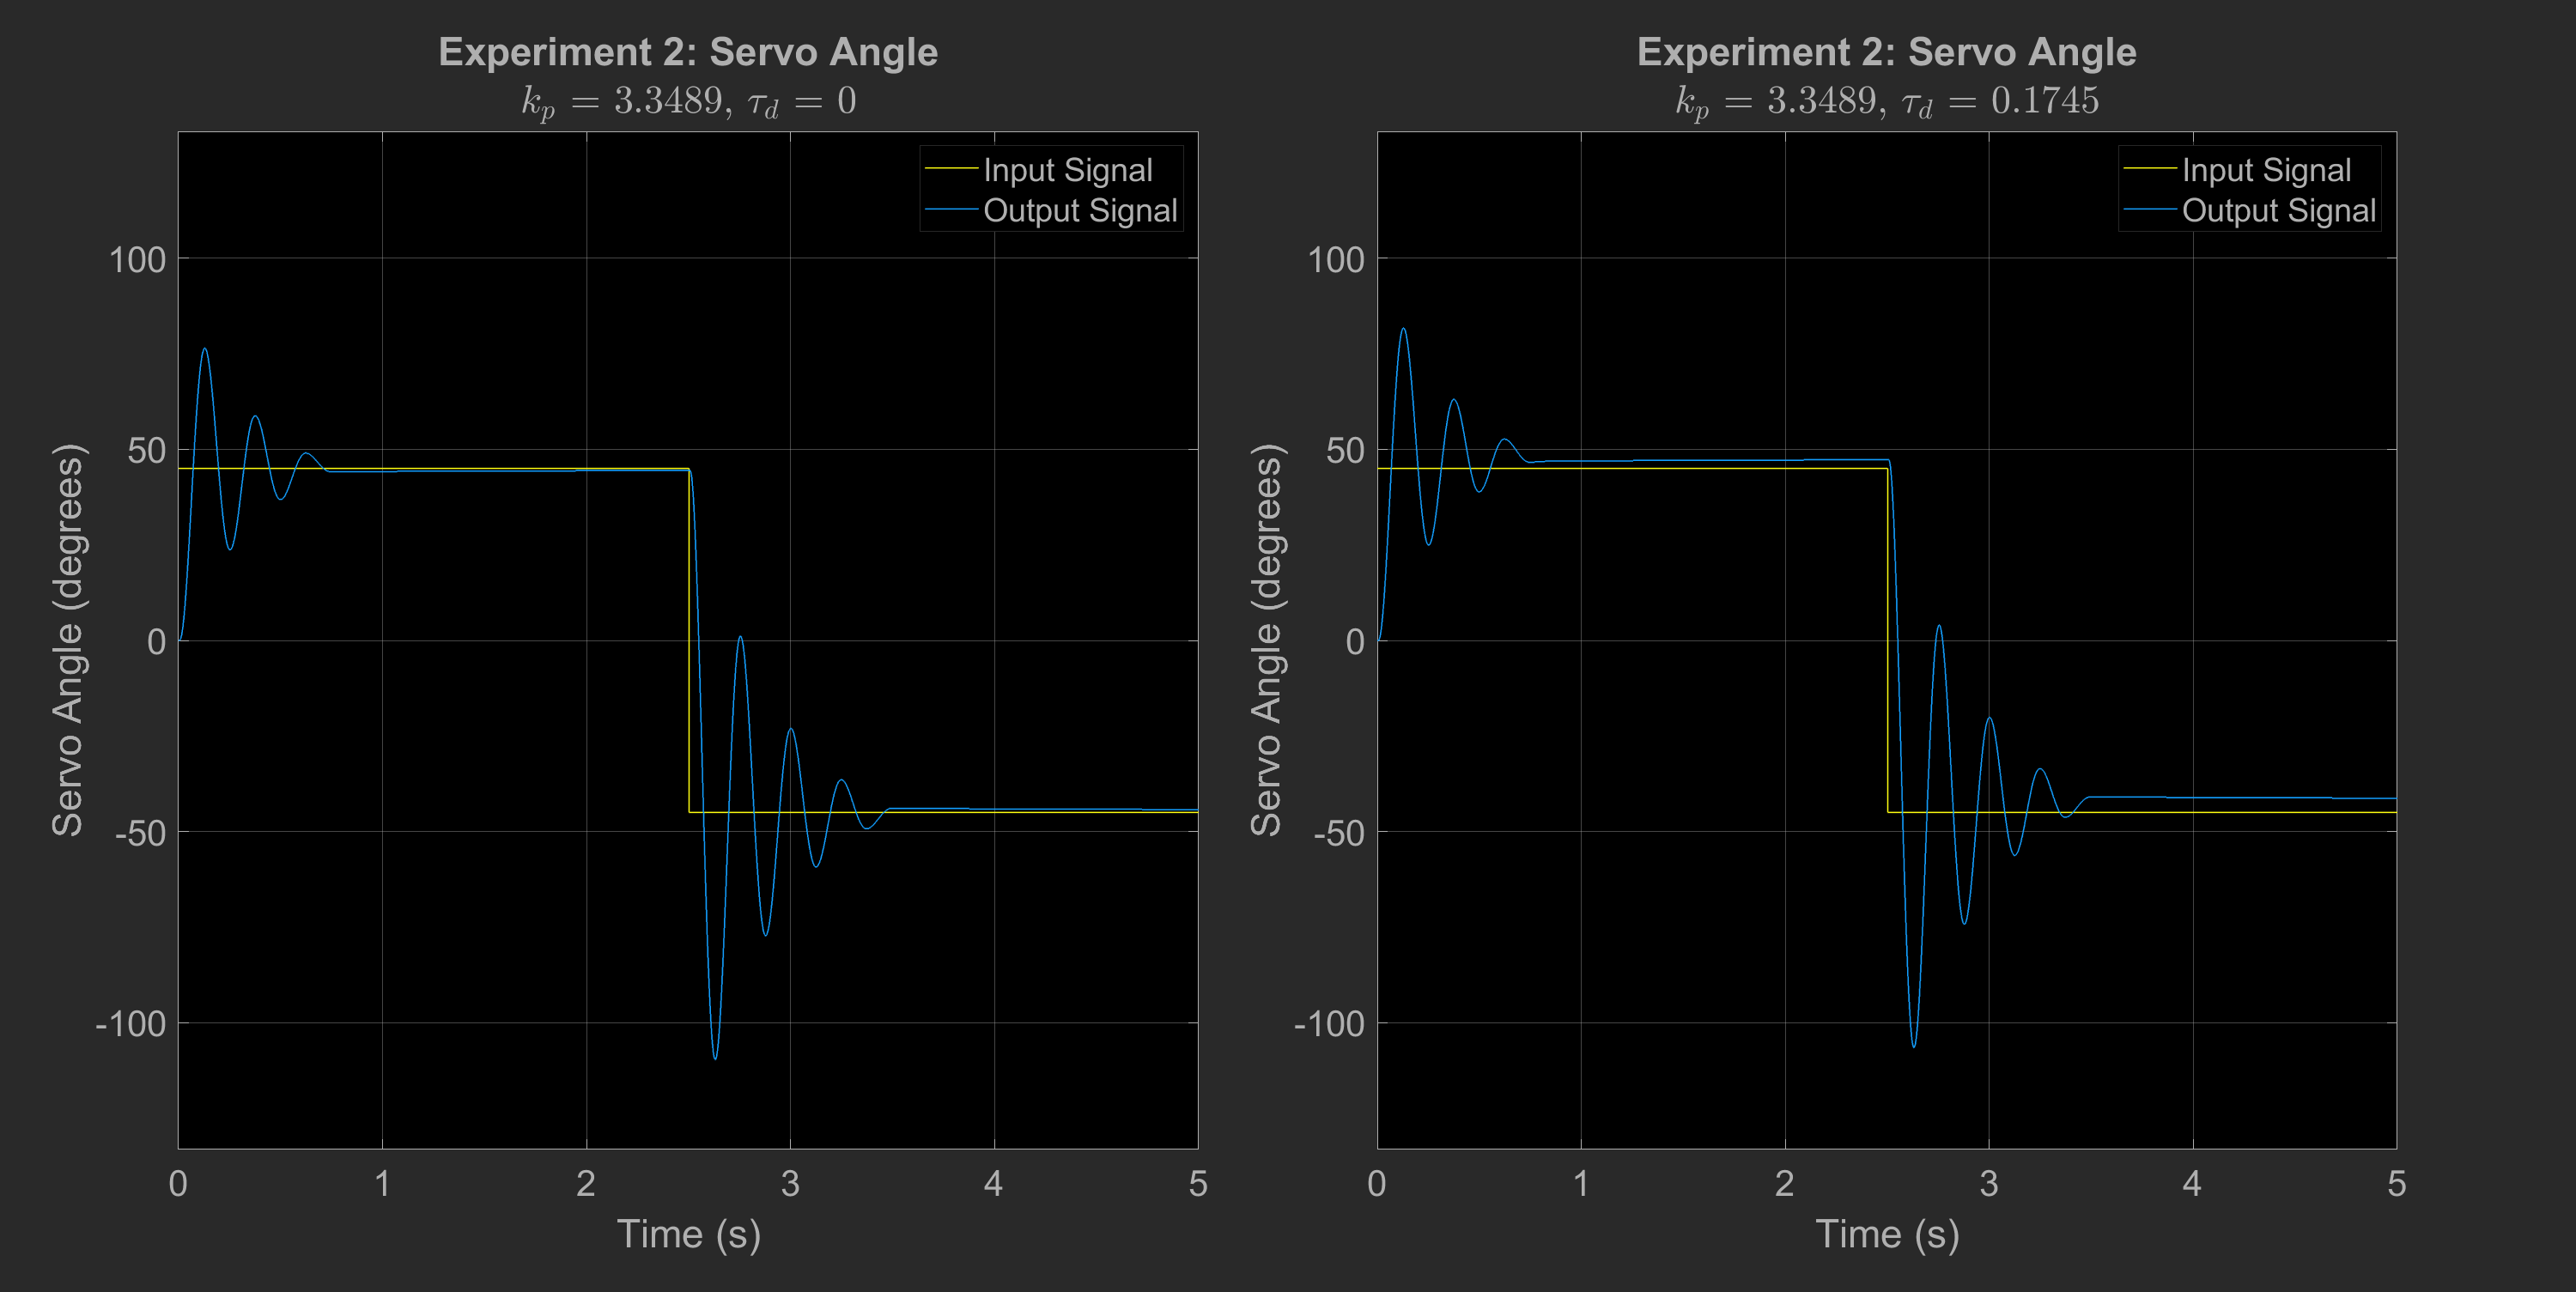
\includegraphics[width=0.91\textwidth]{exp2_kp3.3489}
    \caption{Experiment 2: $k_p = 3.3489$}
\end{figure}

\clearpage
\section{Experiment 3 Figures} \label{appendix:exp3fig}
\begin{figure}[h]
    \centering
    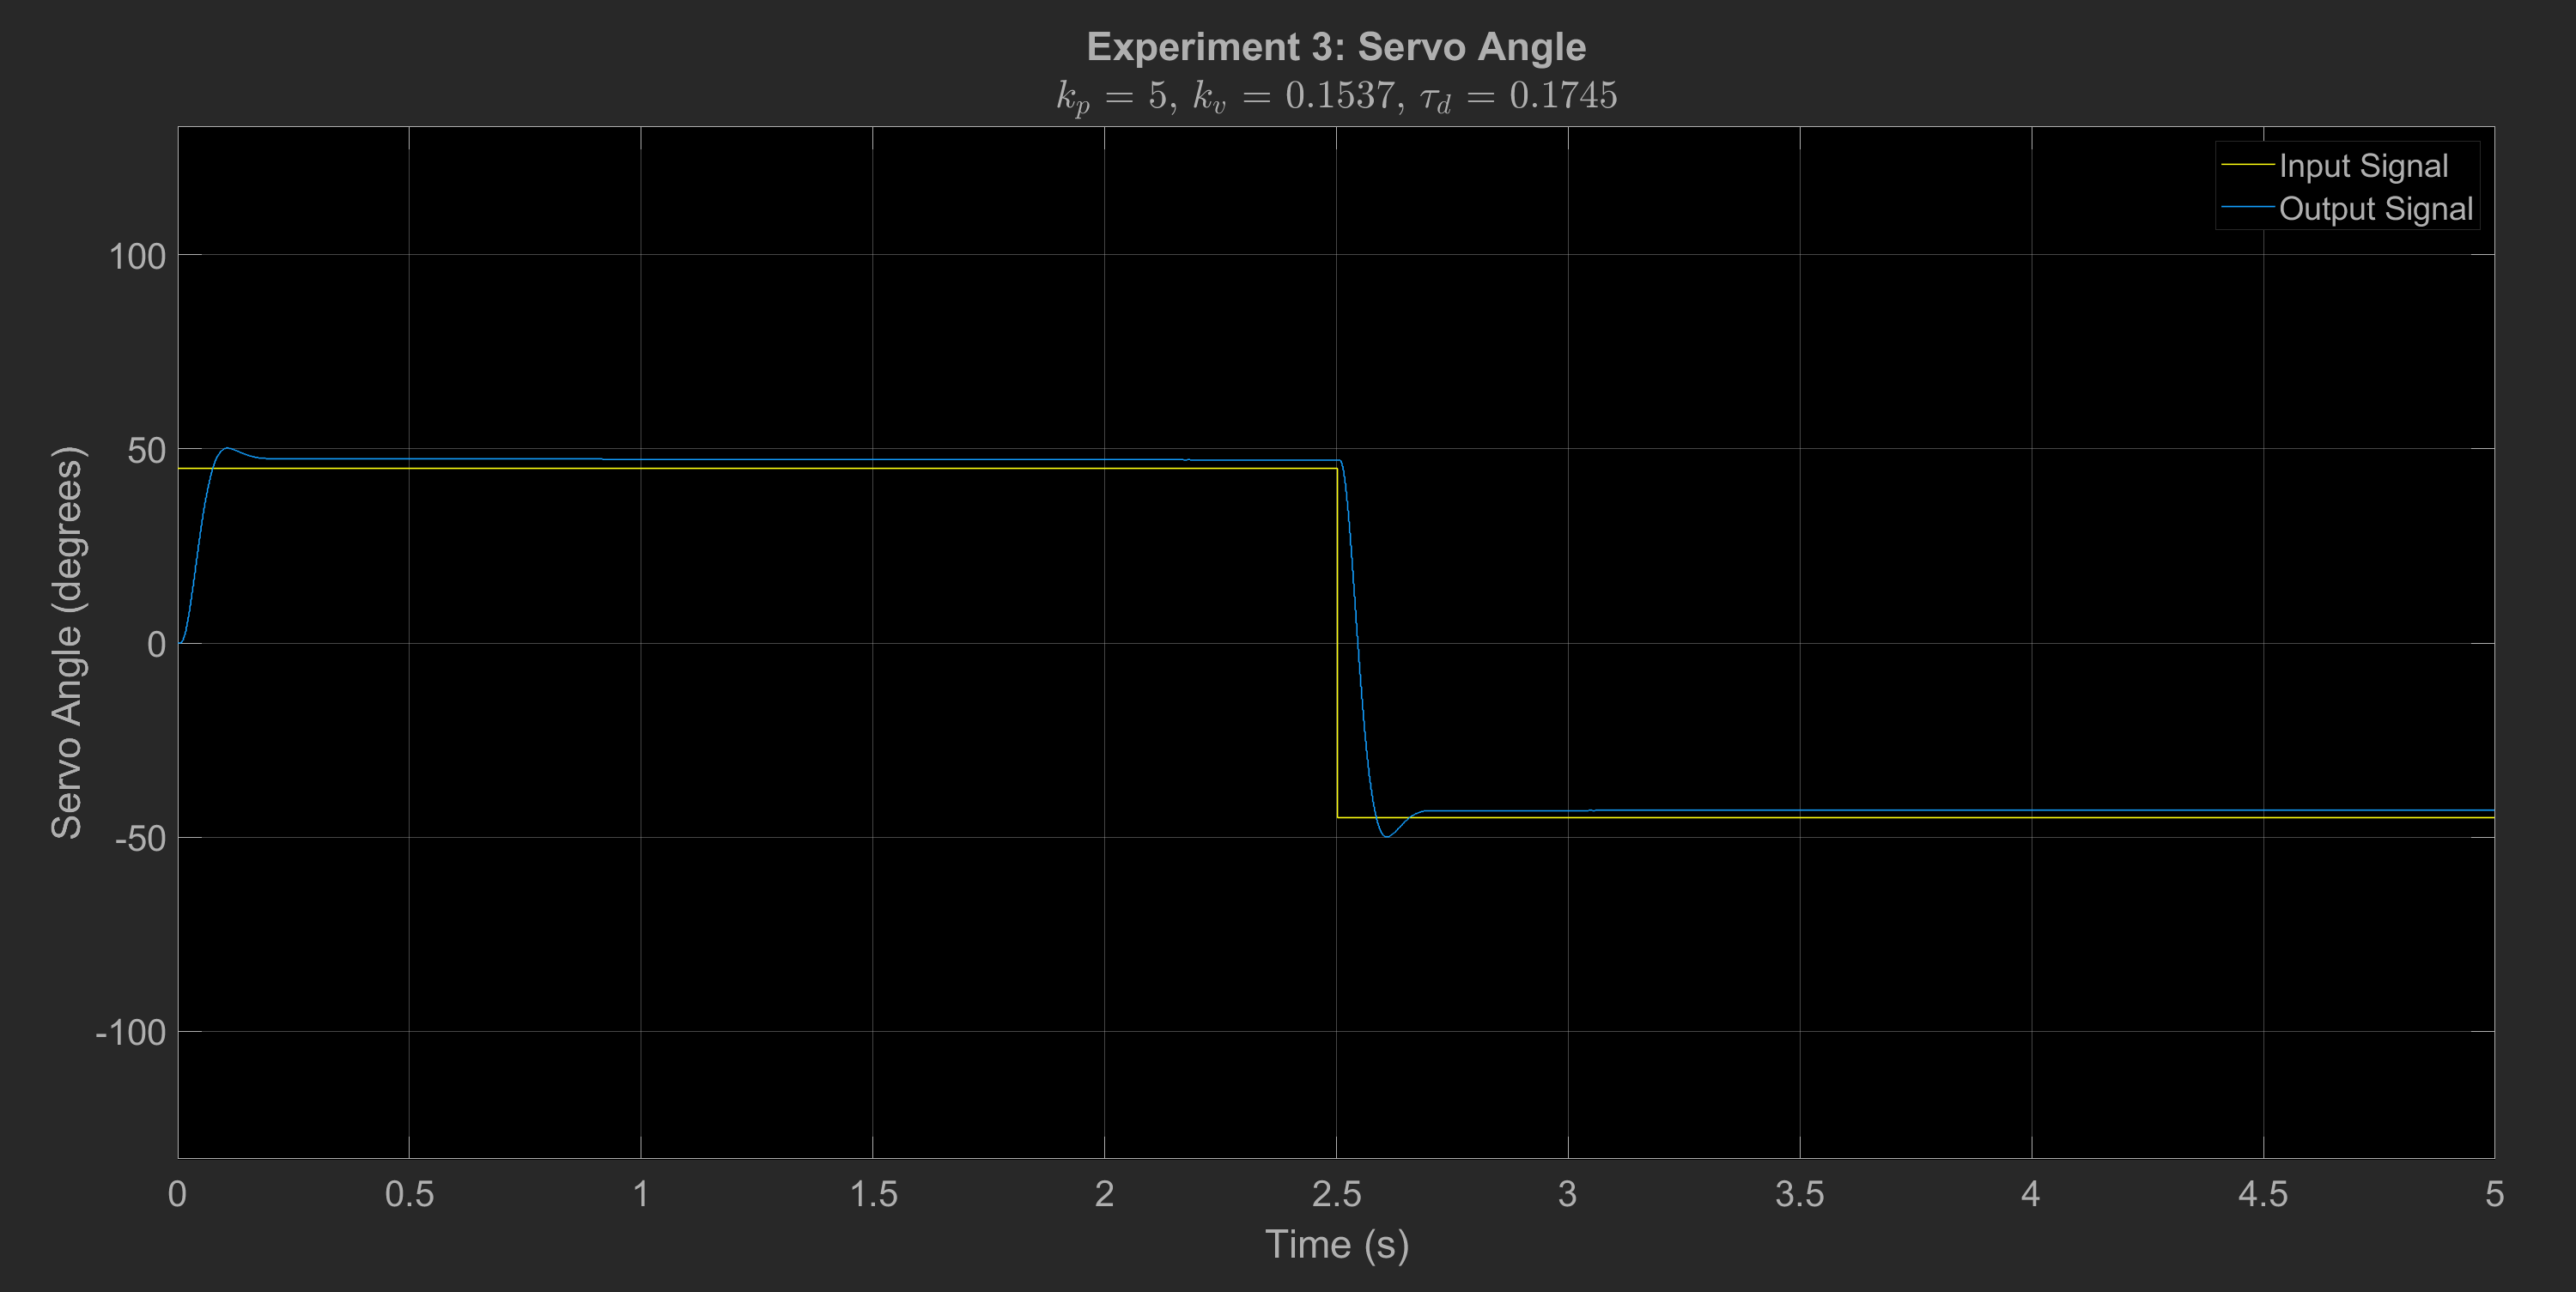
\includegraphics[width=0.91\textwidth]{exp3_kp5_kv0.1537}
    \caption{Experiment 3: $k_p = 5$, $k_v = 0.1537$}
\end{figure}
\begin{figure}[h]
    \centering
    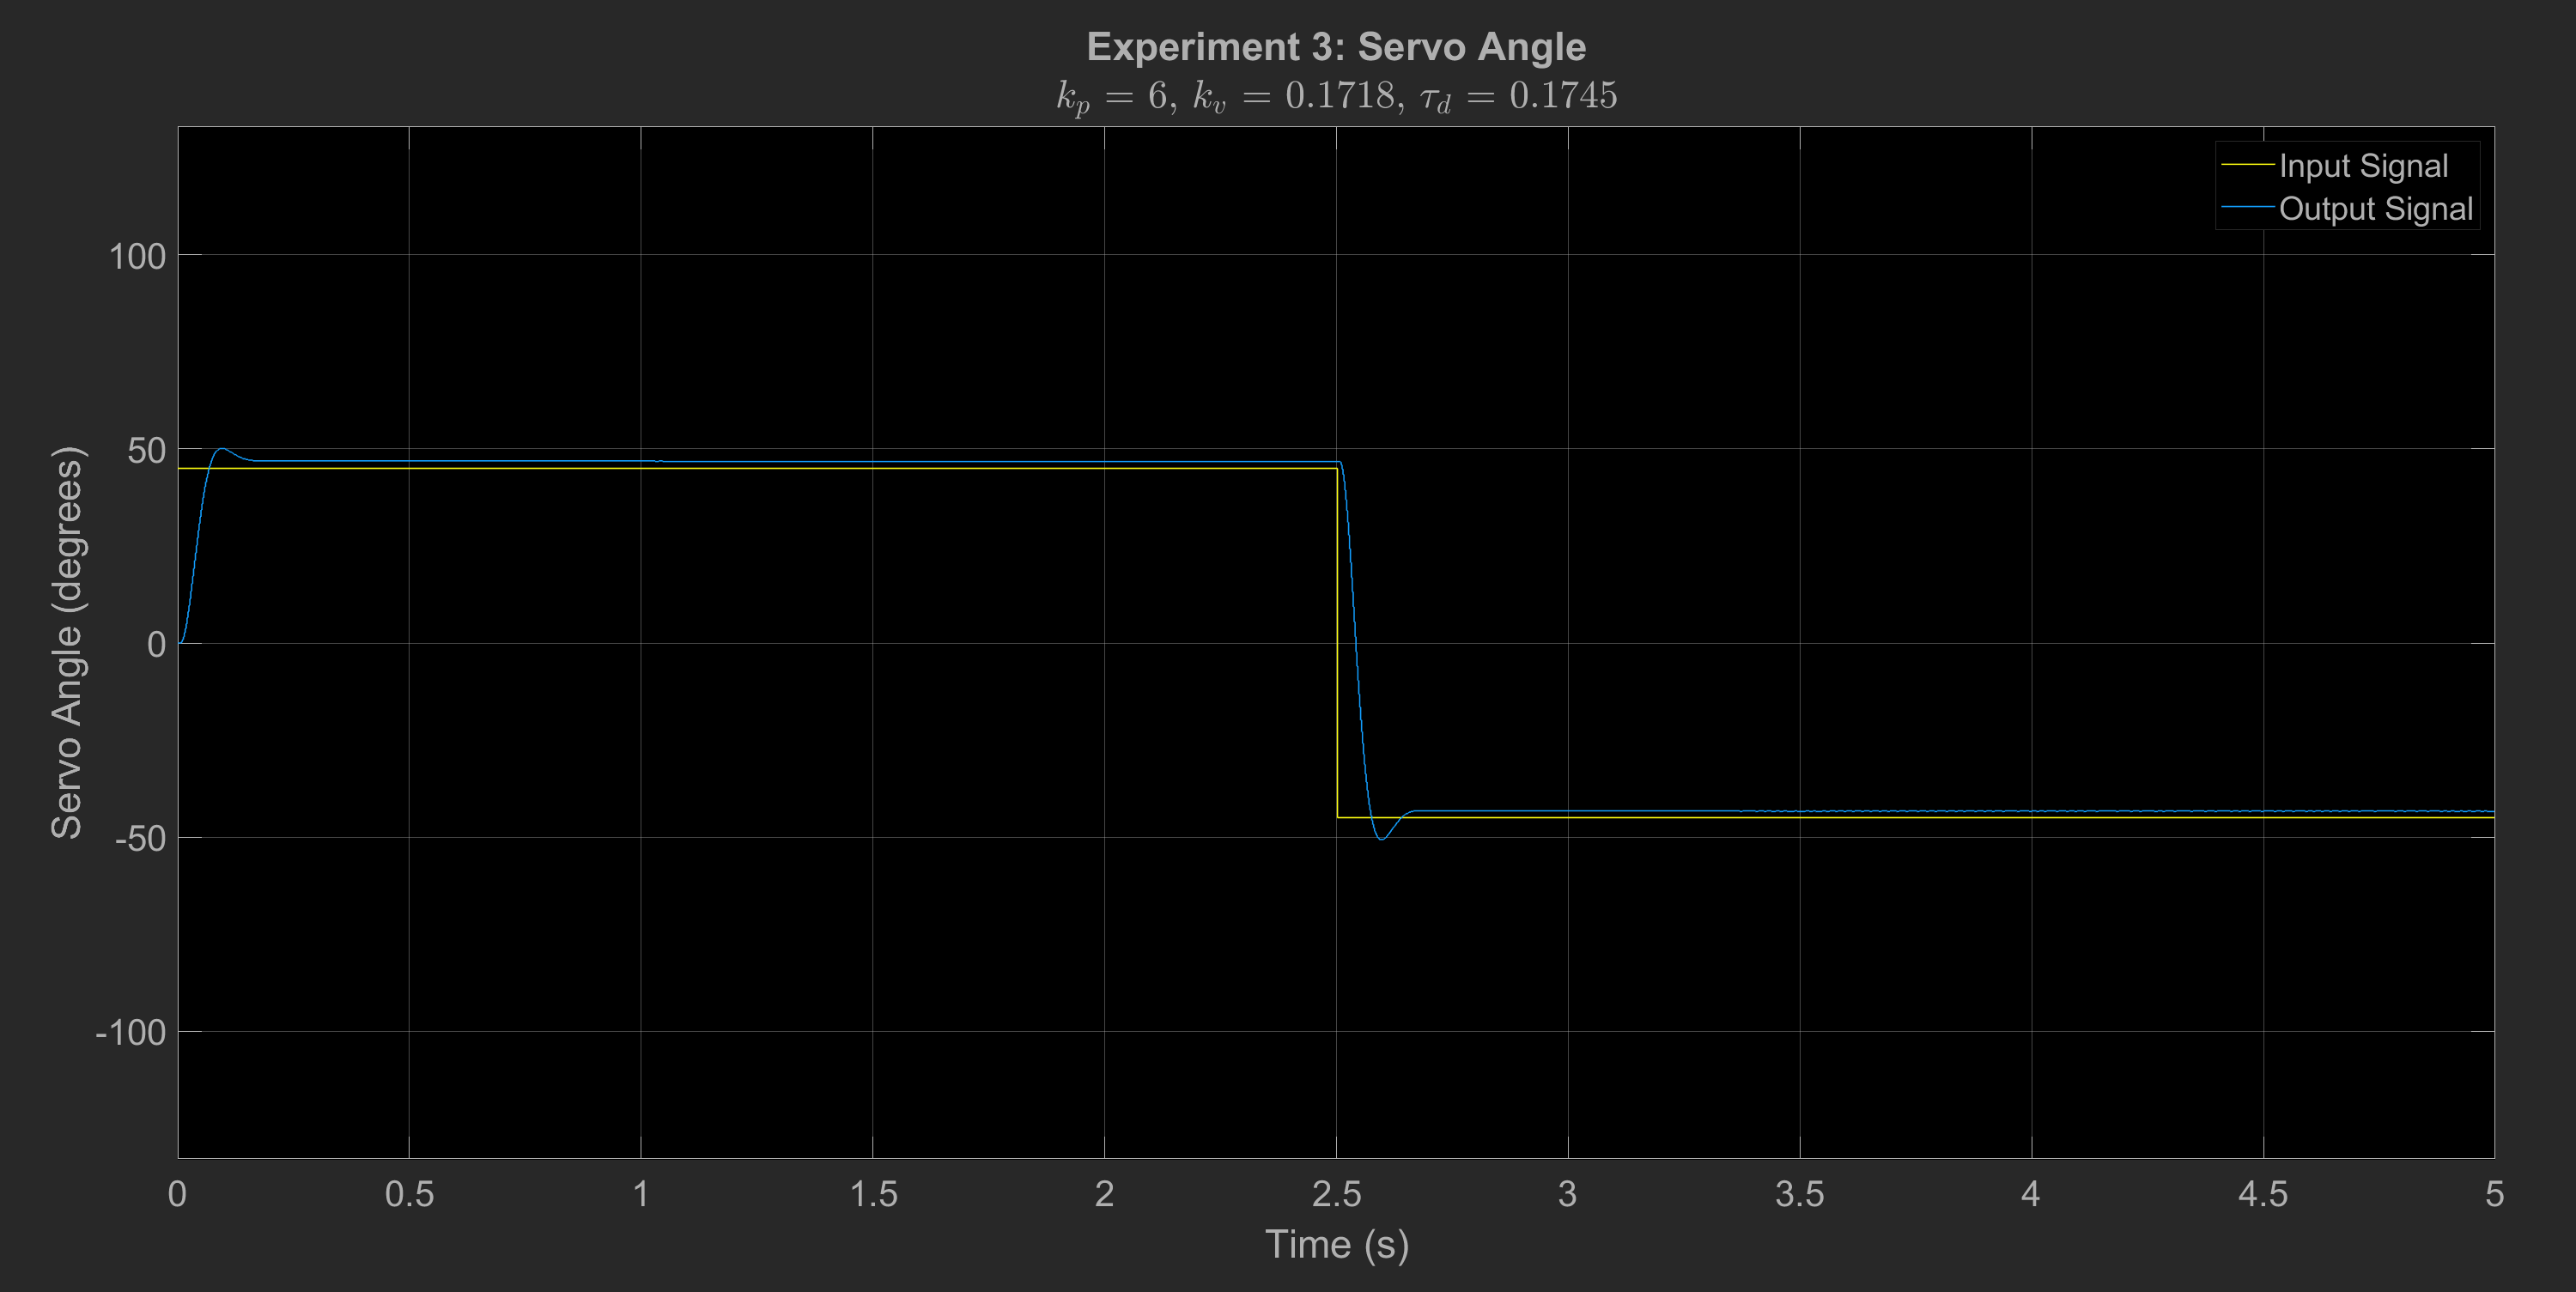
\includegraphics[width=0.91\textwidth]{exp3_kp6_kv0.1718}
    \caption{Experiment 3: $k_p = 6$, $k_v = 0.1718$}
\end{figure}
\begin{figure}[t!]
    \centering
    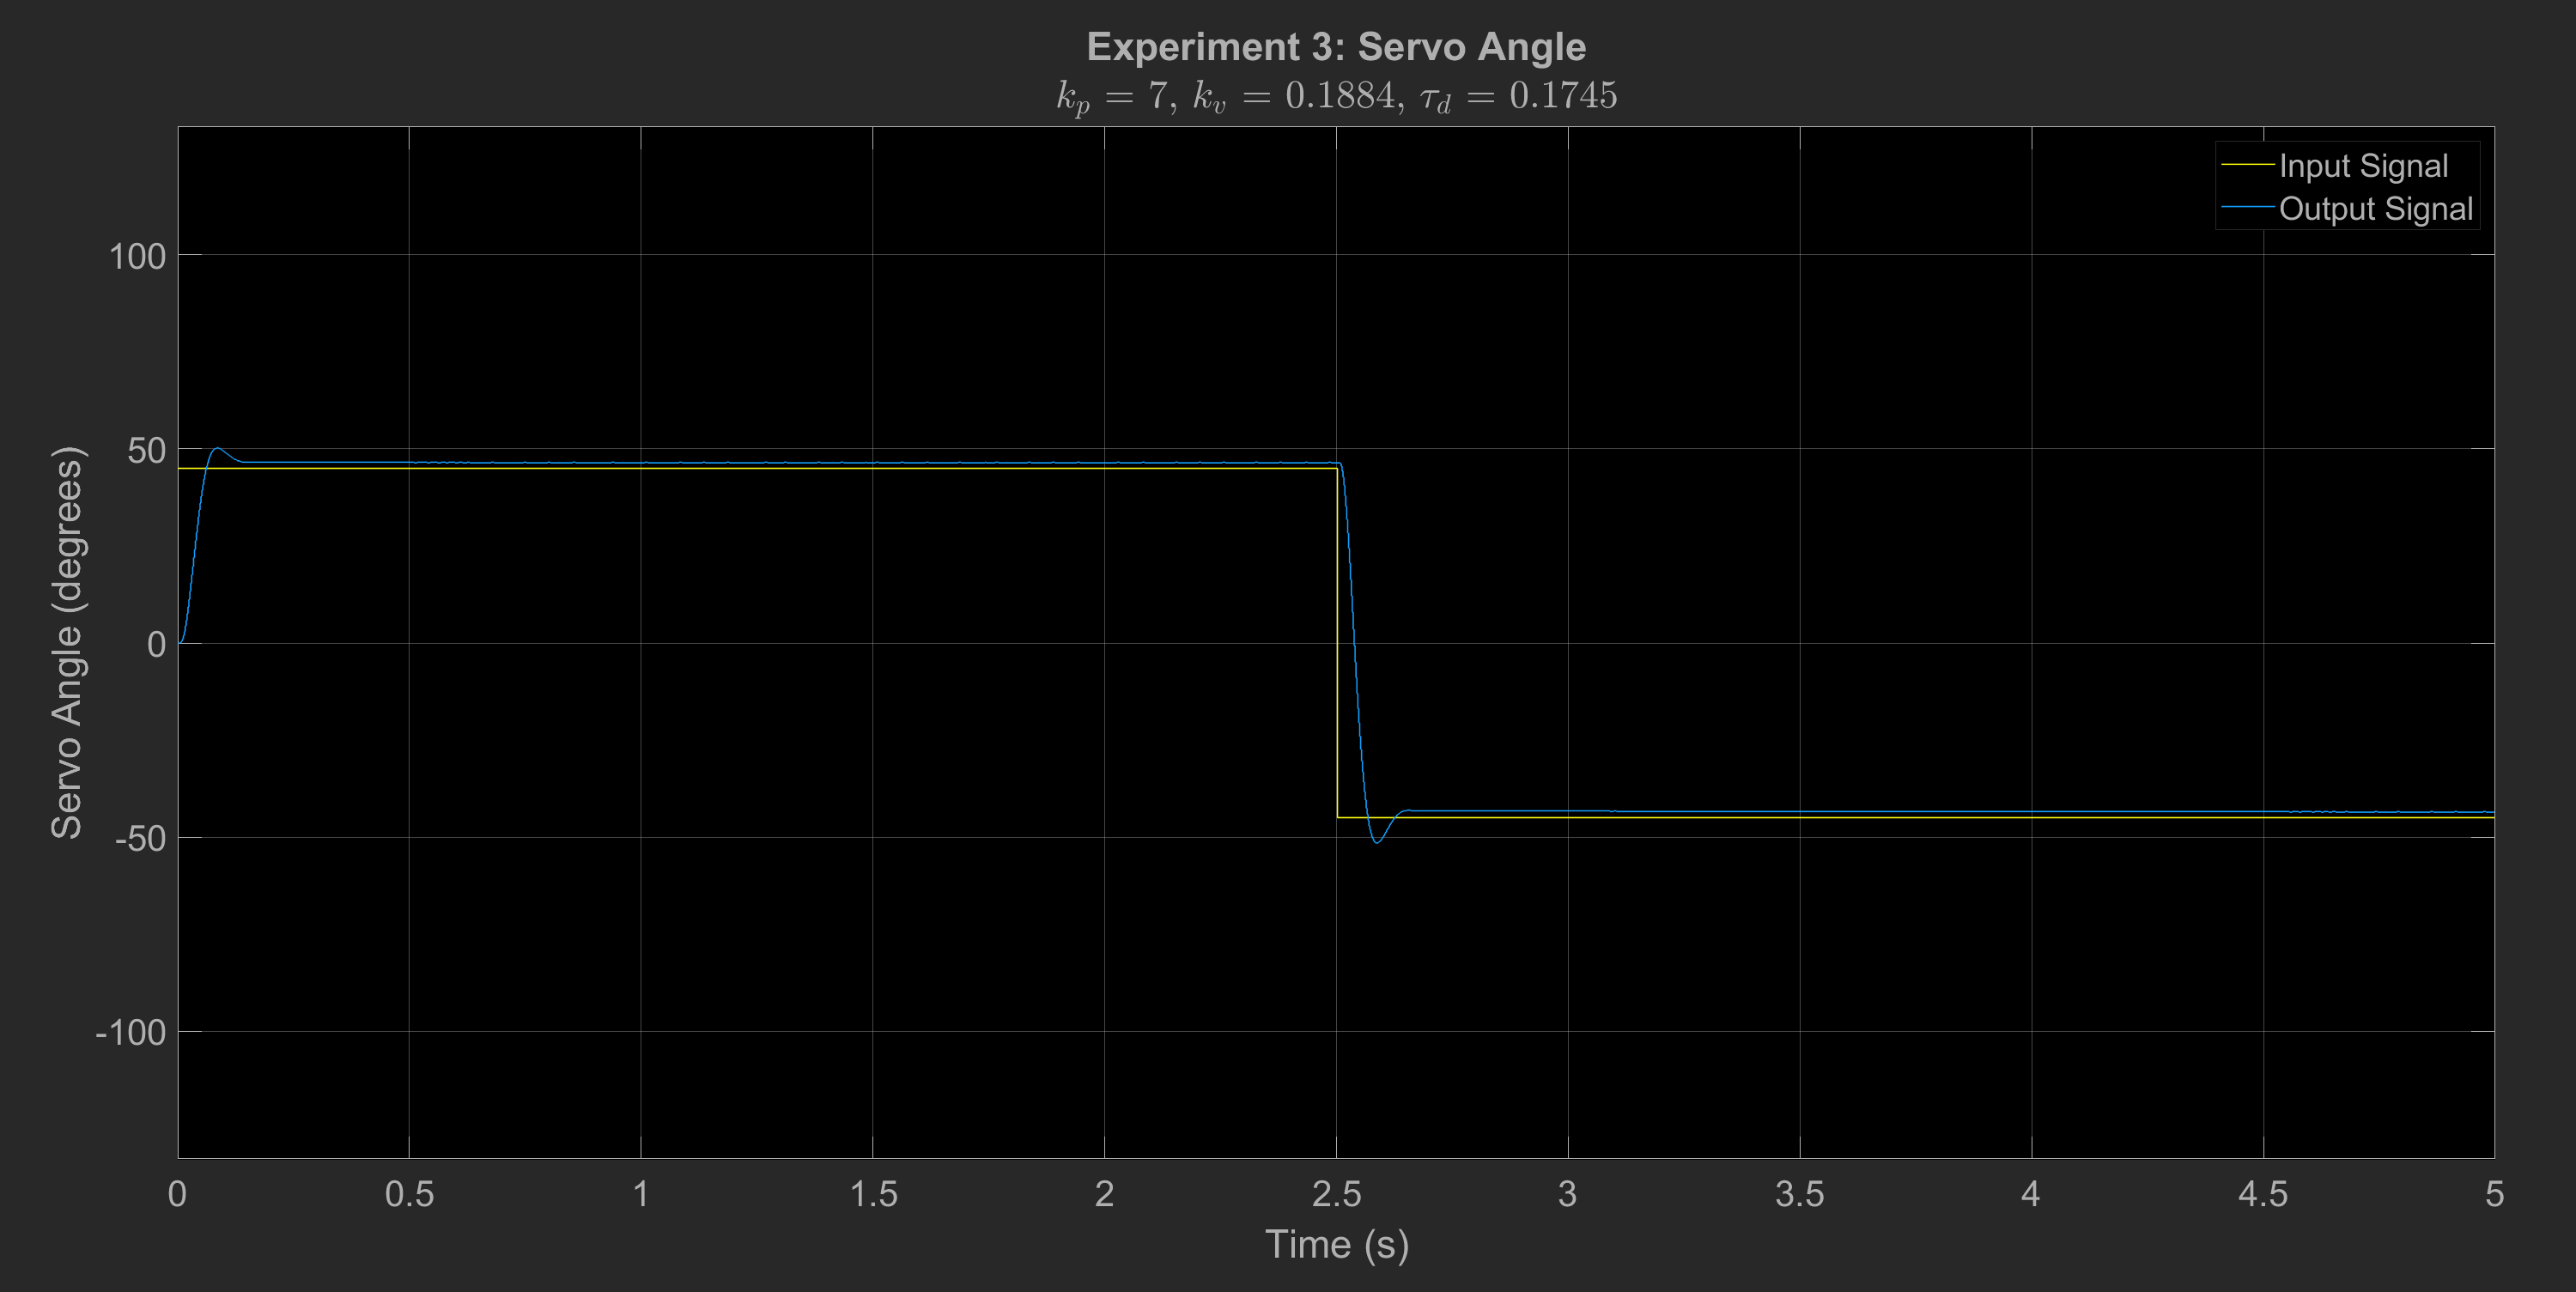
\includegraphics[width=0.91\textwidth]{exp3_kp7_kv0.1884}
    \caption{Experiment 3: $k_p = 7$, $k_v = 0.1884$}
\end{figure}
\end{document}